% Options for packages loaded elsewhere
\PassOptionsToPackage{unicode}{hyperref}
\PassOptionsToPackage{hyphens}{url}
%
\documentclass[
]{book}
\usepackage{amsmath,amssymb}
\usepackage{iftex}
\ifPDFTeX
  \usepackage[T1]{fontenc}
  \usepackage[utf8]{inputenc}
  \usepackage{textcomp} % provide euro and other symbols
\else % if luatex or xetex
  \usepackage{unicode-math} % this also loads fontspec
  \defaultfontfeatures{Scale=MatchLowercase}
  \defaultfontfeatures[\rmfamily]{Ligatures=TeX,Scale=1}
\fi
\usepackage{lmodern}
\ifPDFTeX\else
  % xetex/luatex font selection
\fi
% Use upquote if available, for straight quotes in verbatim environments
\IfFileExists{upquote.sty}{\usepackage{upquote}}{}
\IfFileExists{microtype.sty}{% use microtype if available
  \usepackage[]{microtype}
  \UseMicrotypeSet[protrusion]{basicmath} % disable protrusion for tt fonts
}{}
\makeatletter
\@ifundefined{KOMAClassName}{% if non-KOMA class
  \IfFileExists{parskip.sty}{%
    \usepackage{parskip}
  }{% else
    \setlength{\parindent}{0pt}
    \setlength{\parskip}{6pt plus 2pt minus 1pt}}
}{% if KOMA class
  \KOMAoptions{parskip=half}}
\makeatother
\usepackage{xcolor}
\usepackage{color}
\usepackage{fancyvrb}
\newcommand{\VerbBar}{|}
\newcommand{\VERB}{\Verb[commandchars=\\\{\}]}
\DefineVerbatimEnvironment{Highlighting}{Verbatim}{commandchars=\\\{\}}
% Add ',fontsize=\small' for more characters per line
\usepackage{framed}
\definecolor{shadecolor}{RGB}{248,248,248}
\newenvironment{Shaded}{\begin{snugshade}}{\end{snugshade}}
\newcommand{\AlertTok}[1]{\textcolor[rgb]{0.94,0.16,0.16}{#1}}
\newcommand{\AnnotationTok}[1]{\textcolor[rgb]{0.56,0.35,0.01}{\textbf{\textit{#1}}}}
\newcommand{\AttributeTok}[1]{\textcolor[rgb]{0.13,0.29,0.53}{#1}}
\newcommand{\BaseNTok}[1]{\textcolor[rgb]{0.00,0.00,0.81}{#1}}
\newcommand{\BuiltInTok}[1]{#1}
\newcommand{\CharTok}[1]{\textcolor[rgb]{0.31,0.60,0.02}{#1}}
\newcommand{\CommentTok}[1]{\textcolor[rgb]{0.56,0.35,0.01}{\textit{#1}}}
\newcommand{\CommentVarTok}[1]{\textcolor[rgb]{0.56,0.35,0.01}{\textbf{\textit{#1}}}}
\newcommand{\ConstantTok}[1]{\textcolor[rgb]{0.56,0.35,0.01}{#1}}
\newcommand{\ControlFlowTok}[1]{\textcolor[rgb]{0.13,0.29,0.53}{\textbf{#1}}}
\newcommand{\DataTypeTok}[1]{\textcolor[rgb]{0.13,0.29,0.53}{#1}}
\newcommand{\DecValTok}[1]{\textcolor[rgb]{0.00,0.00,0.81}{#1}}
\newcommand{\DocumentationTok}[1]{\textcolor[rgb]{0.56,0.35,0.01}{\textbf{\textit{#1}}}}
\newcommand{\ErrorTok}[1]{\textcolor[rgb]{0.64,0.00,0.00}{\textbf{#1}}}
\newcommand{\ExtensionTok}[1]{#1}
\newcommand{\FloatTok}[1]{\textcolor[rgb]{0.00,0.00,0.81}{#1}}
\newcommand{\FunctionTok}[1]{\textcolor[rgb]{0.13,0.29,0.53}{\textbf{#1}}}
\newcommand{\ImportTok}[1]{#1}
\newcommand{\InformationTok}[1]{\textcolor[rgb]{0.56,0.35,0.01}{\textbf{\textit{#1}}}}
\newcommand{\KeywordTok}[1]{\textcolor[rgb]{0.13,0.29,0.53}{\textbf{#1}}}
\newcommand{\NormalTok}[1]{#1}
\newcommand{\OperatorTok}[1]{\textcolor[rgb]{0.81,0.36,0.00}{\textbf{#1}}}
\newcommand{\OtherTok}[1]{\textcolor[rgb]{0.56,0.35,0.01}{#1}}
\newcommand{\PreprocessorTok}[1]{\textcolor[rgb]{0.56,0.35,0.01}{\textit{#1}}}
\newcommand{\RegionMarkerTok}[1]{#1}
\newcommand{\SpecialCharTok}[1]{\textcolor[rgb]{0.81,0.36,0.00}{\textbf{#1}}}
\newcommand{\SpecialStringTok}[1]{\textcolor[rgb]{0.31,0.60,0.02}{#1}}
\newcommand{\StringTok}[1]{\textcolor[rgb]{0.31,0.60,0.02}{#1}}
\newcommand{\VariableTok}[1]{\textcolor[rgb]{0.00,0.00,0.00}{#1}}
\newcommand{\VerbatimStringTok}[1]{\textcolor[rgb]{0.31,0.60,0.02}{#1}}
\newcommand{\WarningTok}[1]{\textcolor[rgb]{0.56,0.35,0.01}{\textbf{\textit{#1}}}}
\usepackage{longtable,booktabs,array}
\usepackage{calc} % for calculating minipage widths
% Correct order of tables after \paragraph or \subparagraph
\usepackage{etoolbox}
\makeatletter
\patchcmd\longtable{\par}{\if@noskipsec\mbox{}\fi\par}{}{}
\makeatother
% Allow footnotes in longtable head/foot
\IfFileExists{footnotehyper.sty}{\usepackage{footnotehyper}}{\usepackage{footnote}}
\makesavenoteenv{longtable}
\usepackage{graphicx}
\makeatletter
\def\maxwidth{\ifdim\Gin@nat@width>\linewidth\linewidth\else\Gin@nat@width\fi}
\def\maxheight{\ifdim\Gin@nat@height>\textheight\textheight\else\Gin@nat@height\fi}
\makeatother
% Scale images if necessary, so that they will not overflow the page
% margins by default, and it is still possible to overwrite the defaults
% using explicit options in \includegraphics[width, height, ...]{}
\setkeys{Gin}{width=\maxwidth,height=\maxheight,keepaspectratio}
% Set default figure placement to htbp
\makeatletter
\def\fps@figure{htbp}
\makeatother
\setlength{\emergencystretch}{3em} % prevent overfull lines
\providecommand{\tightlist}{%
  \setlength{\itemsep}{0pt}\setlength{\parskip}{0pt}}
\setcounter{secnumdepth}{5}
\usepackage{booktabs}
\usepackage{amsthm}
\makeatletter
\def\thm@space@setup{%
  \thm@preskip=8pt plus 2pt minus 4pt
  \thm@postskip=\thm@preskip
}
\makeatother
\ifLuaTeX
  \usepackage{selnolig}  % disable illegal ligatures
\fi
\usepackage[]{natbib}
\bibliographystyle{apalike}
\IfFileExists{bookmark.sty}{\usepackage{bookmark}}{\usepackage{hyperref}}
\IfFileExists{xurl.sty}{\usepackage{xurl}}{} % add URL line breaks if available
\urlstyle{same}
\hypersetup{
  pdftitle={Using Spatial Data with R},
  pdfauthor={Claudia A Engel},
  hidelinks,
  pdfcreator={LaTeX via pandoc}}

\title{Using Spatial Data with R}
\author{Claudia A Engel}
\date{Last updated: February 20, 2024}

\begin{document}
\maketitle

{
\setcounter{tocdepth}{1}
\tableofcontents
}
\hypertarget{prerequisites-and-preparations}{%
\chapter*{Prerequisites and Preparations}\label{prerequisites-and-preparations}}
\addcontentsline{toc}{chapter}{Prerequisites and Preparations}

To get the most out of this workshop you should have:

\begin{itemize}
\tightlist
\item
  a \textbf{basic knowledge} of R and/or be familiar with the topics covered in the \href{https://cengel.github.io/R-intro/}{Introduction to R}.
\item
  have a recent version of \href{https://cran.r-project.org/}{R} and \href{https://www.rstudio.com/}{RStudio} installed.
\end{itemize}

\textbf{Recommended}:

\begin{itemize}
\item
  Create a new RStudio project \texttt{R-spatial} in a new folder \texttt{R-spatial}.
\item
  Create a new folder under \texttt{R-spatial} and call it \texttt{data}.
\item
  Open up a new R Script file and call it \texttt{R-spatial.R} for the code you'll create during the workshop.
\item
  If you have your working directory set to \texttt{R-spatial} which contains a folder called \texttt{data} you can copy, paste, and run the following lines in R:
\end{itemize}

\begin{Shaded}
\begin{Highlighting}[]
\FunctionTok{download.file}\NormalTok{(}\StringTok{"http://bit.ly/R{-}spatial{-}data"}\NormalTok{, }\StringTok{"R{-}spatial{-}data.zip"}\NormalTok{)}
\FunctionTok{unzip}\NormalTok{(}\StringTok{"R{-}spatial{-}data.zip"}\NormalTok{, }\AttributeTok{exdir =} \StringTok{"data"}\NormalTok{)}
\end{Highlighting}
\end{Shaded}

You can also download the data manually here \href{https://github.com/cengel/R-spatial/raw/master/data/R-spatial-data.zip}{R-spatial-data.zip} and extract them in the \texttt{data} folder.

\begin{itemize}
\tightlist
\item
  Install and load the following libraries:

  \begin{itemize}
  \tightlist
  \item
    \href{https://cran.r-project.org/package=sf}{\texttt{sf}}
  \item
    \href{https://cran.r-project.org/package=terra}{\texttt{terra}}
  \item
    \href{https://cran.r-project.org/package=tidyverse}{\texttt{tidyverse}}
  \end{itemize}
\item
  For the mapping section install and load these additional libraries:

  \begin{itemize}
  \tightlist
  \item
    \href{https://cran.r-project.org/package=classInt}{\texttt{classInt}}
  \item
    \href{https://cran.r-project.org/package=RColorBrewer}{\texttt{RColorBrewer}}
  \item
    \href{https://cran.r-project.org/package=ggplot2}{\texttt{ggplot2}}
  \item
    \href{https://cran.r-project.org/package=tmap}{\texttt{tmap}}
  \item
    \href{https://cran.r-project.org/package=leaflet}{\texttt{leaflet}}(On Mac installing binary version is ok)
  \end{itemize}
\end{itemize}

\hypertarget{references}{%
\section*{References}\label{references}}
\addcontentsline{toc}{section}{References}

Lovelace, R., Nowosad, J., Muenchow. J. (2024): \href{https://r.geocompx.org/}{Geocomputation with R}

Pebesma, E. Bivand, R. (2023): \href{https://r-spatial.org/book/}{Spatial Data Science}

Gimond, M (2023): \href{https://mgimond.github.io/Spatial/index.html}{Intro to GIS and Spatial Analysis}

\href{http://www.rspatial.org/index.html}{Spatial Data Analysis and Modeling with R and \emph{terra}}

\href{https://CRAN.R-project.org/view=Spatial}{CRAN Task View: Analysis of Spatial Data}

\hypertarget{acknowledgements}{%
\section*{Acknowledgements}\label{acknowledgements}}
\addcontentsline{toc}{section}{Acknowledgements}

Some of the materials for this tutorial are adapted from \url{http://datacarpentry.org}

\hypertarget{intro}{%
\chapter{Introduction to spatial data in R}\label{intro}}

\begin{quote}
Learning Objectives

\begin{itemize}
\tightlist
\item
  Read table with geo coordinates into \texttt{sf} object
\item
  Read shapefiles into \texttt{sf} object
\item
  Examine \texttt{sf} objects
\item
  Use base plot with \texttt{sf} objects and attribute data
\item
  Read GeoTiff single and multiband into a \texttt{SpatRaster} object
\item
  Examine \texttt{SpatRaster} objects
\end{itemize}
\end{quote}

\begin{center}\rule{0.5\linewidth}{0.5pt}\end{center}

\hypertarget{the-sf-package}{%
\section{\texorpdfstring{The \texttt{sf} package}{The sf package}}\label{the-sf-package}}

The \href{https://cran.r-project.org/package=sf}{\texttt{sf}}\footnote{E. Pebesma \& R. Bivand (2016)\href{http://pebesma.staff.ifgi.de/pebesma_sfr.pdf}{Spatial data in R: simple features and
  future perspectives}} package was first released on CRAN in late October 2016, and has in the mean time superseded the original R Package for storing and manipulating spatial data, \href{https://CRAN.R-project.org/package=sp}{\texttt{sp}}, which was first released in 2005. \texttt{sp} is still actively maintained, but less often used now, so you should be aware of it, but we will not teach it here.

\begin{figure}
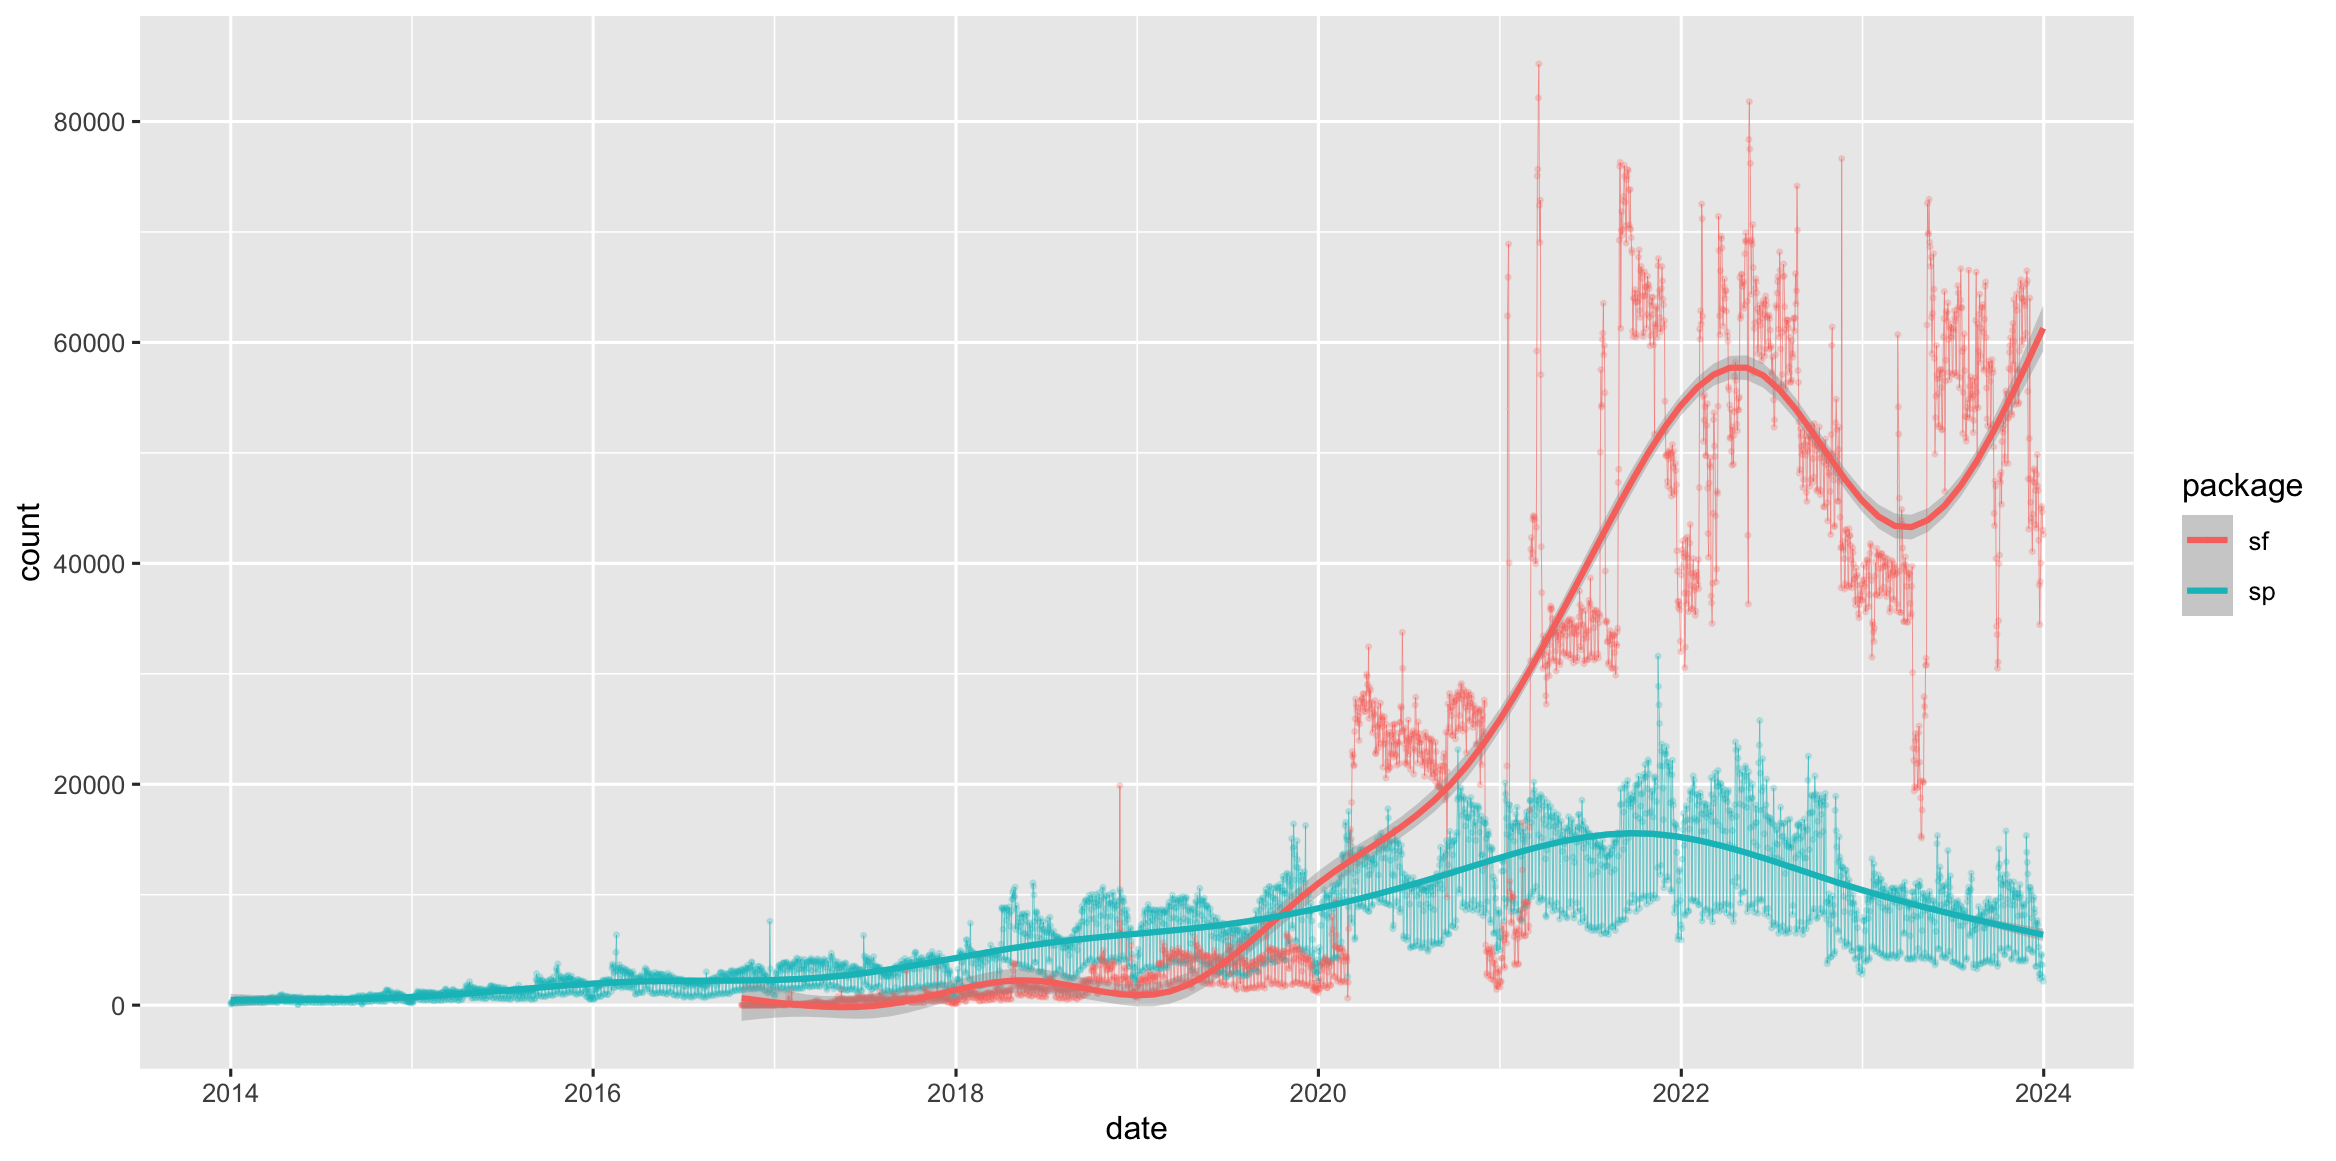
\includegraphics[width=1\linewidth]{img/spsf_downloads} \caption{sf vs sp downloads on CRAN}\label{fig:spsf-dl}
\end{figure}

\texttt{sf} implements a formal standard called \href{https://en.wikipedia.org/wiki/Simple_Features}{``Simple Features''} that specifies a storage and access model of spatial geometries (point, line, polygon). A feature geometry is called simple when it consists of points connected by straight line pieces, and does not intersect itself. This standard has been adopted widely, not only by spatial databases such as PostGIS, but also more recent standards such as GeoJSON.

If you work with PostGis or GeoJSON you may have come across the \href{https://en.wikipedia.org/wiki/Well-known_text}{WKT (well-known text)} format (Fig 1.1 and 1.2)

\begin{figure}
\includegraphics[width=1\linewidth]{img/wkt_primitives} \caption{Well-Known-Text Geometry primitives  (wikipedia)}\label{fig:wkt-primitives}
\end{figure}

\begin{figure}
\includegraphics[width=1\linewidth]{img/wkt_multipart} \caption{Well-Known-Text Multipart geometries (wikipedia)}\label{fig:wkt-multipart}
\end{figure}

\texttt{sf} implements this standard natively in R. In \texttt{sf} spatial objects are stored as a tabular format (data frame) with a special column that contains the information for the geometry coordinates. That special column holds a list with the same length as the number of rows in the data frame. Each of the individual list elements then can be of any length needed to hold the coordinates that correspond to an individual feature.

\texttt{sf} objects are built up using the following structures:

\begin{enumerate}
\def\labelenumi{\arabic{enumi}.}
\tightlist
\item
  \texttt{sfg} - simple feature geometry (one feature)
\item
  \texttt{sfc} - simple feature collection (a collection of \texttt{sfg})
\item
  \texttt{sf} - simple feature object (\texttt{sfc} with data attributes)
\end{enumerate}

So to create a spatial \texttt{sf} object manually the basic steps would be:

\begin{quote}
\textbf{I. Create geometric objects (topology)}
\end{quote}

Geometric objects (simple features) can be created from a numeric vector, matrix or a list with the coordinates. They are called \texttt{sfg} objects for Simple Feature Geometry.b There are functions that help create simple feature geometries, like \texttt{st\_point()}, \texttt{st\_linestring()}, \texttt{st\_polygon()} and more.

\begin{quote}
\textbf{II. Combine all individual single feature objects for the special column.}
\end{quote}

The feature geometries are then combined into a Simple Feature Collection with \texttt{st\_sfc()}. which is nothing other than a simple feature geometry list-column. The \texttt{sfc} object also holds the bounding box and the projection information.

\begin{quote}
\textbf{III. Add attributes}.
\end{quote}

Lastly, we add the attributes to the the simple feature collection with the \texttt{st\_sf()} function. This function extends the well known data frame in R with a column that holds the simple feature collection.

To create a network of highways we would first generate LINESTRINGs as simple feature geometries out of a matrix with coordinates:

\begin{Shaded}
\begin{Highlighting}[]
\NormalTok{lnstr\_sfg1 }\OtherTok{\textless{}{-}} \FunctionTok{st\_linestring}\NormalTok{(}\FunctionTok{matrix}\NormalTok{(}\FunctionTok{runif}\NormalTok{(}\DecValTok{6}\NormalTok{), }\AttributeTok{ncol=}\DecValTok{2}\NormalTok{)) }
\NormalTok{lnstr\_sfg2 }\OtherTok{\textless{}{-}} \FunctionTok{st\_linestring}\NormalTok{(}\FunctionTok{matrix}\NormalTok{(}\FunctionTok{runif}\NormalTok{(}\DecValTok{6}\NormalTok{), }\AttributeTok{ncol=}\DecValTok{2}\NormalTok{)) }
\FunctionTok{class}\NormalTok{(lnstr\_sfg1)}
\end{Highlighting}
\end{Shaded}

\begin{verbatim}
#> [1] "XY"         "LINESTRING" "sfg"
\end{verbatim}

We would then combine this into a simple feature collection :

\begin{Shaded}
\begin{Highlighting}[]
\NormalTok{(lnstr\_sfc }\OtherTok{\textless{}{-}} \FunctionTok{st\_sfc}\NormalTok{(lnstr\_sfg1, lnstr\_sfg2)) }
\end{Highlighting}
\end{Shaded}

\begin{verbatim}
#> Geometry set for 2 features 
#> Geometry type: LINESTRING
#> Dimension:     XY
#> Bounding box:  xmin: 0.235151 ymin: 0.00839848 xmax: 0.9894396 ymax: 0.6266413
#> CRS:           NA
\end{verbatim}

\begin{verbatim}
#> LINESTRING (0.8592813 0.00839848, 0.9273943 0.3...
\end{verbatim}

\begin{verbatim}
#> LINESTRING (0.235151 0.2268521, 0.9894396 0.350...
\end{verbatim}

And lastly create a data frame from above to generate the \texttt{sf} object:

\begin{Shaded}
\begin{Highlighting}[]
\NormalTok{dfr }\OtherTok{\textless{}{-}} \FunctionTok{data.frame}\NormalTok{(}\AttributeTok{id =} \FunctionTok{c}\NormalTok{(}\StringTok{"hwy1"}\NormalTok{, }\StringTok{"hwy2"}\NormalTok{), }
                  \AttributeTok{cars\_per\_hour =} \FunctionTok{c}\NormalTok{(}\DecValTok{78}\NormalTok{, }\DecValTok{22}\NormalTok{))}
\NormalTok{(lnstr\_sf }\OtherTok{\textless{}{-}} \FunctionTok{st\_sf}\NormalTok{(dfr , lnstr\_sfc))}
\end{Highlighting}
\end{Shaded}

\begin{verbatim}
#> Simple feature collection with 2 features and 2 fields
#> Geometry type: LINESTRING
#> Dimension:     XY
#> Bounding box:  xmin: 0.235151 ymin: 0.00839848 xmax: 0.9894396 ymax: 0.6266413
#> CRS:           NA
#>     id cars_per_hour                      lnstr_sfc
#> 1 hwy1            78 LINESTRING (0.8592813 0.008...
#> 2 hwy2            22 LINESTRING (0.235151 0.2268...
\end{verbatim}

There are many methods available in the \texttt{sf} package, to find out use

\begin{Shaded}
\begin{Highlighting}[]
\FunctionTok{methods}\NormalTok{(}\AttributeTok{class=}\StringTok{"sf"}\NormalTok{)}
\end{Highlighting}
\end{Shaded}

\begin{verbatim}
#>   [1] [                            [[<-                        
#>   [3] [<-                          $<-                         
#>   [5] aggregate                    anti_join                   
#>   [7] arrange                      as.data.frame               
#>   [9] cbind                        coerce                      
#>  [11] crs                          dbDataType                  
#>  [13] dbWriteTable                 distance                    
#>  [15] distinct                     dplyr_reconstruct           
#>  [17] drop_na                      duplicated                  
#>  [19] ext                          extract                     
#>  [21] filter                       full_join                   
#>  [23] gather                       group_by                    
#>  [25] group_split                  identify                    
#>  [27] initialize                   inner_join                  
#>  [29] left_join                    lines                       
#>  [31] mask                         merge                       
#>  [33] mutate                       nest                        
#>  [35] pivot_longer                 pivot_wider                 
#>  [37] plot                         points                      
#>  [39] polys                        print                       
#>  [41] rasterize                    rbind                       
#>  [43] rename_with                  rename                      
#>  [45] right_join                   rowwise                     
#>  [47] sample_frac                  sample_n                    
#>  [49] select                       semi_join                   
#>  [51] separate_rows                separate                    
#>  [53] show                         slice                       
#>  [55] slotsFromS3                  spread                      
#>  [57] st_agr                       st_agr<-                    
#>  [59] st_area                      st_as_s2                    
#>  [61] st_as_sf                     st_as_sfc                   
#>  [63] st_bbox                      st_boundary                 
#>  [65] st_break_antimeridian        st_buffer                   
#>  [67] st_cast                      st_centroid                 
#>  [69] st_collection_extract        st_concave_hull             
#>  [71] st_convex_hull               st_coordinates              
#>  [73] st_crop                      st_crs                      
#>  [75] st_crs<-                     st_difference               
#>  [77] st_drop_geometry             st_filter                   
#>  [79] st_geometry                  st_geometry<-               
#>  [81] st_inscribed_circle          st_interpolate_aw           
#>  [83] st_intersection              st_intersects               
#>  [85] st_is_valid                  st_is                       
#>  [87] st_join                      st_line_merge               
#>  [89] st_m_range                   st_make_valid               
#>  [91] st_minimum_rotated_rectangle st_nearest_points           
#>  [93] st_node                      st_normalize                
#>  [95] st_point_on_surface          st_polygonize               
#>  [97] st_precision                 st_reverse                  
#>  [99] st_sample                    st_segmentize               
#> [101] st_set_precision             st_shift_longitude          
#> [103] st_simplify                  st_snap                     
#> [105] st_sym_difference            st_transform                
#> [107] st_triangulate_constrained   st_triangulate              
#> [109] st_union                     st_voronoi                  
#> [111] st_wrap_dateline             st_write                    
#> [113] st_z_range                   st_zm                       
#> [115] summarise                    svc                         
#> [117] transform                    transmute                   
#> [119] ungroup                      unite                       
#> [121] unnest                       vect                        
#> see '?methods' for accessing help and source code
\end{verbatim}

Here are some of the other highlights of \texttt{sf} you might be interested in:

\begin{itemize}
\tightlist
\item
  provides \textbf{fast} I/O, particularly relevant for large files
\item
  spatial functions that rely on GEOS and GDAL and PROJ external libraries are directly linked into the package, so no need to load additional external packages (like in \texttt{sp})
\item
  \texttt{sf} objects can be plotted directly with \texttt{ggplot}
\item
  \texttt{sf} directly reads from and writes to spatial \textbf{databases} such as PostGIS
\item
  \texttt{sf} is compatible with the \href{https://www.tidyverse.org/}{\texttt{tidyvderse} approach}, (but see some \href{https://geocompr.github.io/geocompkg/articles/tidyverse-pitfalls.html}{pitfalls here})
\end{itemize}

Note that \texttt{sp} and \texttt{sf} are not the only way spatial objects are conceptualized in R. Other spatial packages may use their own class definitions for spatial data (for example \texttt{spatstat}).

There are packages specifically for the \href{https://tools.ietf.org/html/rfc7946}{GeoJSON} and for that reason are more lightweight, for example \href{https://cran.r-project.org/package=geojson}{\texttt{geojson}}

Usually you can find functions that convert objects to and from these formats.

\begin{quote}
Challenge

Generate an \texttt{sf} point object.

\begin{enumerate}
\def\labelenumi{\arabic{enumi}.}
\tightlist
\item
  Create a matrix \texttt{pts} of random numbers with two columns and as many rows as you like. These are your points.
\item
  Create a dataframe \texttt{attrib\_df} with the same number of rows as your \texttt{pts} matrix and a column that holds an attribute. You can make up any attribute.
\item
  Use the appropriate commands and \texttt{pts} an \texttt{sf} object with a gemoetry column of class \texttt{sfc\_POINT}.
\item
  Try to subset your spatial object using the attribute you have added and the way you are used to from regular data frames.
\item
  How do you determine the bounding box of your spatial object?
\end{enumerate}
\end{quote}

\hypertarget{creating-a-spatial-object-from-a-latlon-table}{%
\section{Creating a spatial object from a lat/lon table}\label{creating-a-spatial-object-from-a-latlon-table}}

Often in your research might have a spreadsheet that contains latitude, longitude and perhaps some attribute values. You know how to read the spreadsheet into a tabular format (tibble) with \texttt{dplyr::read\_table} or \texttt{dplyr::read\_csv}. We can then very easily convert the table into a spatial object in R.

An \texttt{sf} object can be created from a data frame in the following way. We take advantage of the \texttt{st\_as\_sf()} function which converts any foreign object into an \texttt{sf} object. Similarly to above, it requires an argument \texttt{coords}, which in the case of point data needs to be a vector that specifies the data frame's columns for the longitude and latitude (x,y) coordinates.

\begin{verbatim}
my_sf_object <- st_as_sf(myDataframe, coords)
\end{verbatim}

\texttt{st\_as\_sf()} creates a new object and leaves the original data frame untouched.

We use \texttt{read\_csv()} to read \texttt{philly\_homicides.csv} into a tibble in R and name it \texttt{philly\_homicides\_df}.

\begin{Shaded}
\begin{Highlighting}[]
\NormalTok{philly\_homicides\_df }\OtherTok{\textless{}{-}} \FunctionTok{read\_csv}\NormalTok{(}\StringTok{"data/philly\_homicides.csv"}\NormalTok{)}
\end{Highlighting}
\end{Shaded}

\begin{verbatim}
#> Rows: 3883 Columns: 10
#> -- Column specification --------------------------------------------------------
#> Delimiter: ","
#> chr  (3): SECTOR, LOCATION_BLOCK, TEXT_GENERAL_CODE
#> dbl  (5): DC_DIST, UCR_GENERAL, OBJ_ID, POINT_X, POINT_Y
#> date (1): DISPATCH_DATE
#> time (1): DISPATCH_TIME
#> 
#> i Use `spec()` to retrieve the full column specification for this data.
#> i Specify the column types or set `show_col_types = FALSE` to quiet this message.
\end{verbatim}

We convert the \texttt{philly\_homicides\_df} data frame into an \texttt{sf} object with \texttt{st\_as\_sf()}

\begin{Shaded}
\begin{Highlighting}[]
\FunctionTok{library}\NormalTok{(sf)}

\NormalTok{philly\_homicides\_sf }\OtherTok{\textless{}{-}} \FunctionTok{st\_as\_sf}\NormalTok{(philly\_homicides\_df, }\AttributeTok{coords =} \FunctionTok{c}\NormalTok{(}\StringTok{"POINT\_X"}\NormalTok{, }\StringTok{"POINT\_Y"}\NormalTok{))}
\FunctionTok{names}\NormalTok{(philly\_homicides\_sf)}
\end{Highlighting}
\end{Shaded}

\begin{verbatim}
#> [1] "DC_DIST"           "SECTOR"            "DISPATCH_DATE"    
#> [4] "DISPATCH_TIME"     "LOCATION_BLOCK"    "UCR_GENERAL"      
#> [7] "OBJ_ID"            "TEXT_GENERAL_CODE" "geometry"
\end{verbatim}

Note the additional \textbf{geometry} list-column which now holds the simple feature collection with the coordinates of all the points. We now use \texttt{st\_crs()} to check on the projection.

\begin{Shaded}
\begin{Highlighting}[]
\FunctionTok{st\_crs}\NormalTok{(philly\_homicides\_sf)}
\end{Highlighting}
\end{Shaded}

\begin{verbatim}
#> Coordinate Reference System: NA
\end{verbatim}

To make it a complete geographical object we use \texttt{st\_crs()} to assign the WGS84 projection, which has the EPSG code 4326:

\begin{Shaded}
\begin{Highlighting}[]
\FunctionTok{st\_crs}\NormalTok{(philly\_homicides\_sf) }\OtherTok{\textless{}{-}} \DecValTok{4326}
\FunctionTok{st\_crs}\NormalTok{(philly\_homicides\_sf)}
\end{Highlighting}
\end{Shaded}

\begin{verbatim}
#> Coordinate Reference System:
#>   User input: EPSG:4326 
#>   wkt:
#> GEOGCRS["WGS 84",
#>     ENSEMBLE["World Geodetic System 1984 ensemble",
#>         MEMBER["World Geodetic System 1984 (Transit)"],
#>         MEMBER["World Geodetic System 1984 (G730)"],
#>         MEMBER["World Geodetic System 1984 (G873)"],
#>         MEMBER["World Geodetic System 1984 (G1150)"],
#>         MEMBER["World Geodetic System 1984 (G1674)"],
#>         MEMBER["World Geodetic System 1984 (G1762)"],
#>         MEMBER["World Geodetic System 1984 (G2139)"],
#>         ELLIPSOID["WGS 84",6378137,298.257223563,
#>             LENGTHUNIT["metre",1]],
#>         ENSEMBLEACCURACY[2.0]],
#>     PRIMEM["Greenwich",0,
#>         ANGLEUNIT["degree",0.0174532925199433]],
#>     CS[ellipsoidal,2],
#>         AXIS["geodetic latitude (Lat)",north,
#>             ORDER[1],
#>             ANGLEUNIT["degree",0.0174532925199433]],
#>         AXIS["geodetic longitude (Lon)",east,
#>             ORDER[2],
#>             ANGLEUNIT["degree",0.0174532925199433]],
#>     USAGE[
#>         SCOPE["Horizontal component of 3D system."],
#>         AREA["World."],
#>         BBOX[-90,-180,90,180]],
#>     ID["EPSG",4326]]
\end{verbatim}

Wow this is long. It is usually more helpful to just retrieve the proj4string:

\begin{Shaded}
\begin{Highlighting}[]
\FunctionTok{st\_crs}\NormalTok{(philly\_homicides\_sf)}\SpecialCharTok{$}\NormalTok{proj4string}
\end{Highlighting}
\end{Shaded}

\begin{verbatim}
#> [1] "+proj=longlat +datum=WGS84 +no_defs"
\end{verbatim}

We will save this object as a shapefile on our hard drive for later use. (Note that by default \texttt{st\_write} checks if the file already exists, and if so it will not overwrite it. If you need to force it to overwrite use the option \texttt{delete\_layer\ =\ TRUE}.)

\begin{Shaded}
\begin{Highlighting}[]
\FunctionTok{st\_write}\NormalTok{(philly\_homicides\_sf, }\StringTok{"data/PhillyHomicides"}\NormalTok{, }\AttributeTok{driver =} \StringTok{"ESRI Shapefile"}\NormalTok{)}
\CommentTok{\# to force the save: }
\FunctionTok{st\_write}\NormalTok{(philly\_homicides\_sf, }\StringTok{"data/PhillyHomicides"}\NormalTok{, }\AttributeTok{driver =} \StringTok{"ESRI Shapefile"}\NormalTok{, }\AttributeTok{delete\_layer =} \ConstantTok{TRUE}\NormalTok{)}
\end{Highlighting}
\end{Shaded}

\hypertarget{loading-shape-files-into-r}{%
\section{Loading shape files into R}\label{loading-shape-files-into-r}}

\texttt{sf} relies on the powerful \href{http://gdal.org}{GDAL library}, which is automatically linked in when loading \texttt{sf}. The GDAL provides the functionality to read and write spatial files of many formats. For shape files we can use \texttt{st\_read()}, which simply takes the path of the directory with the shapefile as argument.

\begin{Shaded}
\begin{Highlighting}[]
\CommentTok{\# read in}
\NormalTok{philly\_sf }\OtherTok{\textless{}{-}} \FunctionTok{st\_read}\NormalTok{(}\StringTok{"data/Philly/"}\NormalTok{)}
\end{Highlighting}
\end{Shaded}

\begin{verbatim}
#> Reading layer `PhillyTotalPopHHinc' from data source 
#>   `/Users/cengel/Anthro/R_Class/R_Workshops/R-spatial/data/Philly' 
#>   using driver `ESRI Shapefile'
#> Simple feature collection with 384 features and 17 fields
#> Geometry type: MULTIPOLYGON
#> Dimension:     XY
#> Bounding box:  xmin: 1739497 ymin: 457343.7 xmax: 1764030 ymax: 490544.9
#> Projected CRS: Albers
\end{verbatim}

\begin{Shaded}
\begin{Highlighting}[]
\CommentTok{\# take a look at what we\textquotesingle{}ve got}
\FunctionTok{str}\NormalTok{(philly\_sf) }\CommentTok{\# note again the geometry column}
\end{Highlighting}
\end{Shaded}

\begin{verbatim}
#> Classes 'sf' and 'data.frame':   384 obs. of  18 variables:
#>  $ STATEFP10 : chr  "42" "42" "42" "42" ...
#>  $ COUNTYFP10: chr  "101" "101" "101" "101" ...
#>  $ TRACTCE10 : chr  "036301" "036400" "036600" "034803" ...
#>  $ GEOID10   : num  4.21e+10 4.21e+10 4.21e+10 4.21e+10 4.21e+10 ...
#>  $ NAME10    : chr  "363.01" "364" "366" "348.03" ...
#>  $ NAMELSAD10: chr  "Census Tract 363.01" "Census Tract 364" "Census Tract 366" "Census Tract 348.03" ...
#>  $ MTFCC10   : chr  "G5020" "G5020" "G5020" "G5020" ...
#>  $ FUNCSTAT10: chr  "S" "S" "S" "S" ...
#>  $ ALAND10   : num  2322732 4501110 1004313 1271533 1016206 ...
#>  $ AWATER10  : num  66075 8014 1426278 8021 0 ...
#>  $ INTPTLAT10: chr  "+40.0895349" "+40.1127747" "+39.9470272" "+40.0619427" ...
#>  $ INTPTLON10: chr  "-074.9667387" "-074.9789137" "-075.1404472" "-075.0023705" ...
#>  $ GISJOIN   : chr  "G4201010036301" "G4201010036400" "G4201010036600" "G4201010034803" ...
#>  $ Shape_area: num  2388806 4509124 2430591 1279556 1016207 ...
#>  $ Shape_len : num  6851 10567 9257 4928 5920 ...
#>  $ medHHinc  : num  54569 NA 130139 56667 69981 ...
#>  $ totalPop  : num  3695 703 1643 4390 3807 ...
#>  $ geometry  :sfc_MULTIPOLYGON of length 384; first list element: List of 1
#>   ..$ :List of 1
#>   .. ..$ : num [1:55, 1:2] 1763647 1763473 1763366 1763378 1763321 ...
#>   ..- attr(*, "class")= chr [1:3] "XY" "MULTIPOLYGON" "sfg"
#>  - attr(*, "sf_column")= chr "geometry"
#>  - attr(*, "agr")= Factor w/ 3 levels "constant","aggregate",..: NA NA NA NA NA NA NA NA NA NA ...
#>   ..- attr(*, "names")= chr [1:17] "STATEFP10" "COUNTYFP10" "TRACTCE10" "GEOID10" ...
\end{verbatim}

Two more words about the geometry column: Though it is not recommended, you can name this column any way you wish. Secondly, you can remove this column and revert to a regular, non-spatial data frame at any dime with \texttt{st\_drop\_geometry()}.

The default \texttt{plot} of an \texttt{sf} object is a multi-plot of the first attributes, with a warning if not all can be plotted:

\begin{Shaded}
\begin{Highlighting}[]
\FunctionTok{plot}\NormalTok{(philly\_sf)}
\end{Highlighting}
\end{Shaded}

\begin{verbatim}
#> Warning: plotting the first 10 out of 17 attributes; use max.plot = 17 to plot
#> all
\end{verbatim}

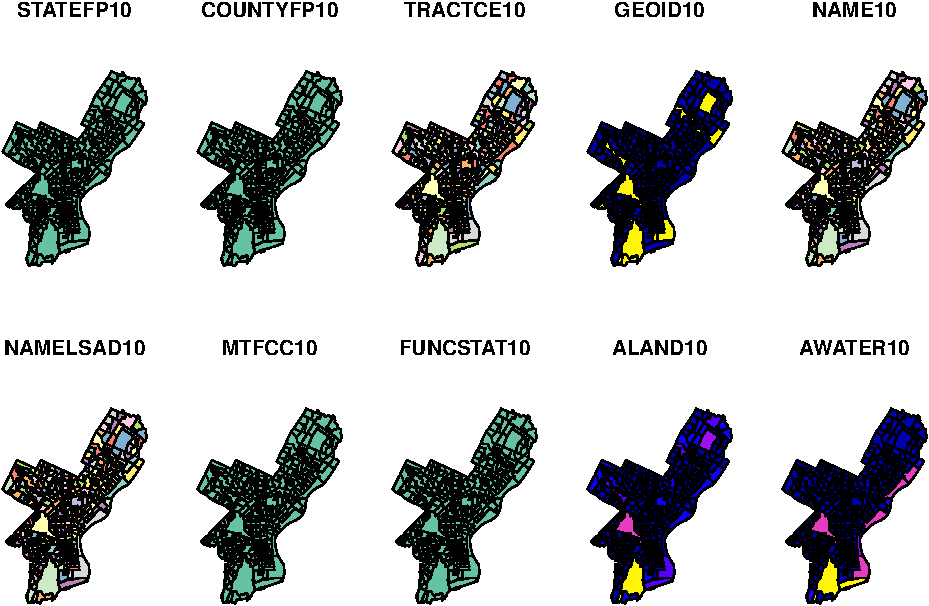
\includegraphics{R-spatial_files/figure-latex/plot-shp-sf-1.pdf}

In order to only plot the polygon boundaries we need to directly use the geometry column. We use the \texttt{st\_geometry()} function. It extracts the \texttt{sfc} object (the simple feature geometry list column):

\begin{Shaded}
\begin{Highlighting}[]
\FunctionTok{plot}\NormalTok{(}\FunctionTok{st\_geometry}\NormalTok{(philly\_sf))}
\end{Highlighting}
\end{Shaded}

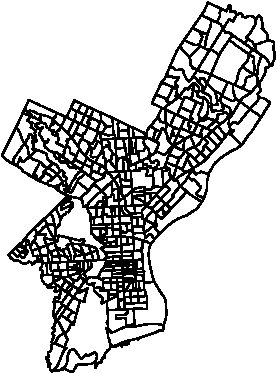
\includegraphics{R-spatial_files/figure-latex/plot-shp-sfg-1.pdf}

Let's add a subset of polygons with only the census tracts where the median houshold income (\emph{medHHinc}) is more than \$60,000. We can extract elements from an \texttt{sf} object based on attributes using the dplyr filter function (base R subsetting also works) and add the census tracts to the plot in a different color.

\begin{Shaded}
\begin{Highlighting}[]
\FunctionTok{plot}\NormalTok{(}\FunctionTok{st\_geometry}\NormalTok{(philly\_sf))}
\NormalTok{philly\_sf }\SpecialCharTok{\%\textgreater{}\%} 
  \FunctionTok{filter}\NormalTok{(medHHinc }\SpecialCharTok{\textgreater{}} \DecValTok{60000}\NormalTok{) }\SpecialCharTok{\%\textgreater{}\%} \CommentTok{\# filter for high income}
  \FunctionTok{st\_geometry}\NormalTok{() }\SpecialCharTok{\%\textgreater{}\%} \CommentTok{\# extract the geometry for plotting}
  \FunctionTok{plot}\NormalTok{(}\AttributeTok{col=}\StringTok{"red"}\NormalTok{, }\AttributeTok{add=}\NormalTok{T) }\CommentTok{\# add to the plot}
\end{Highlighting}
\end{Shaded}

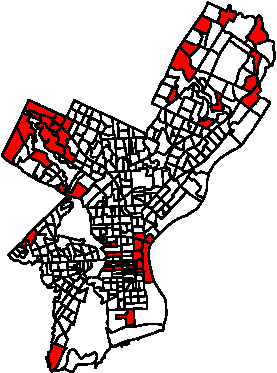
\includegraphics{R-spatial_files/figure-latex/pipe-subset-plot-shp-sfg-1.pdf}

\hypertarget{raster-data-in-r}{%
\section{Raster data in R}\label{raster-data-in-r}}

Raster files, as you might know, have a more compact data structure than vectors. Because of their regular structure the coordinates do not need to be recorded for each pixel or cell in the rectangular extent. A raster is defined by:

\begin{itemize}
\tightlist
\item
  a CRS
\item
  coordinates of its origin
\item
  a distance or cell size in each direction
\item
  a dimension or numbers of cells in each direction
\item
  an array of cell values
\end{itemize}

Given this structure, coordinates for any cell can be computed and don't need to be stored.

\texttt{terra} was first released in 2020 and now replaces the \texttt{raster} package which was first released in 2010. \texttt{terra} has greater functionality, is faster and easier to use.

\begin{figure}
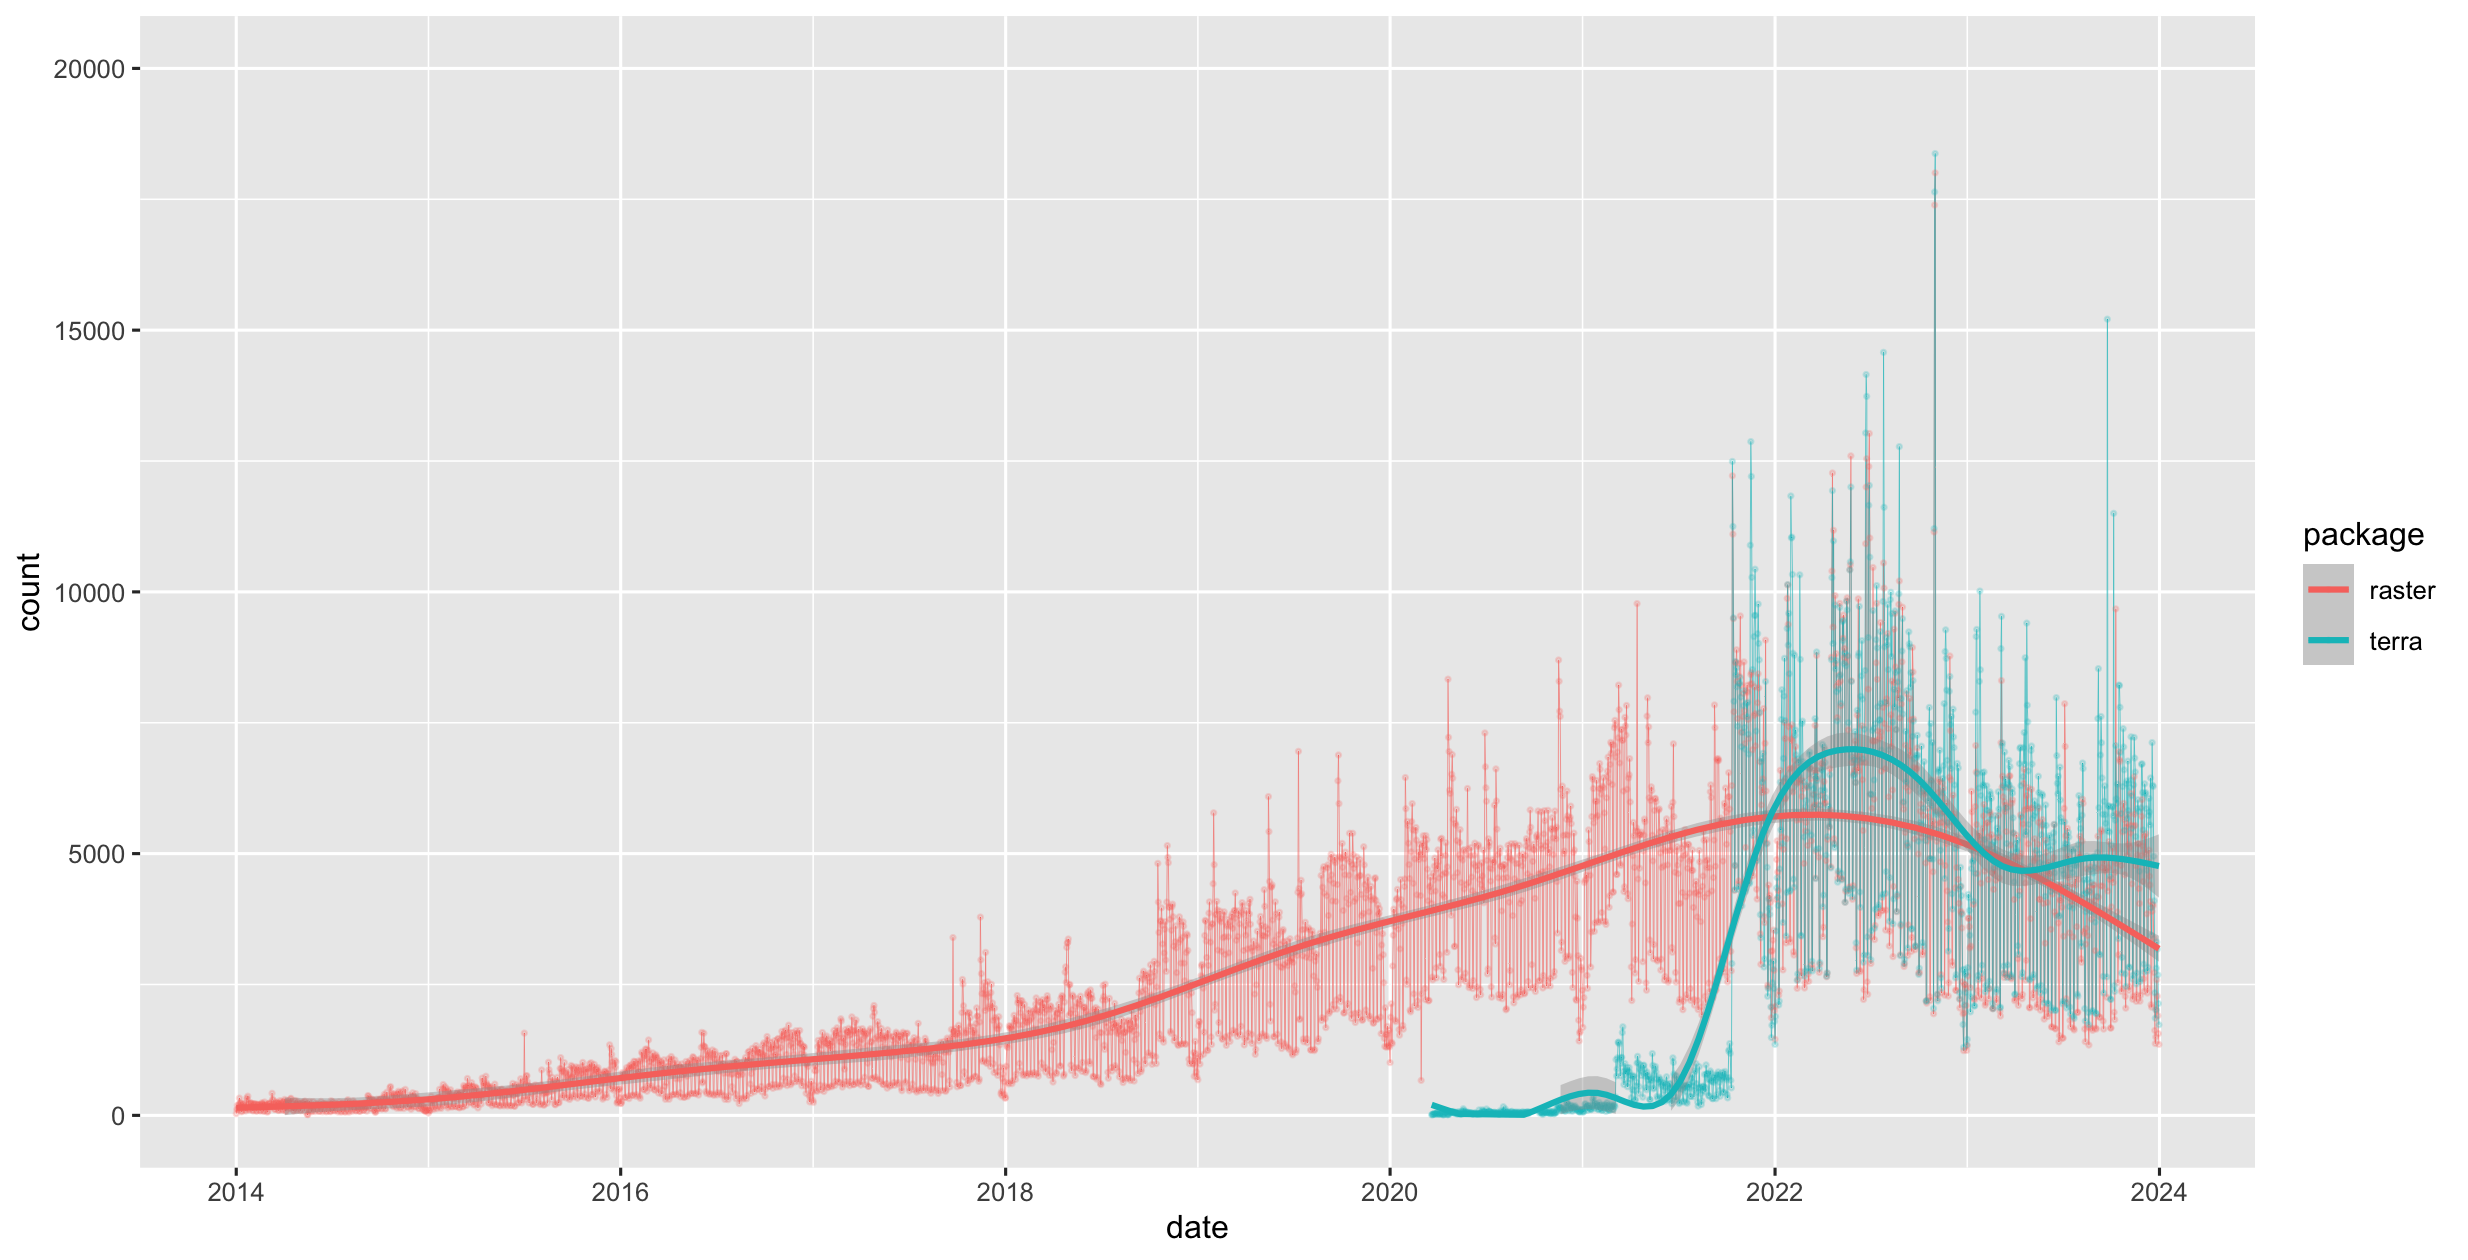
\includegraphics[width=1\linewidth]{img/raster_terraDownloads} \caption{raster vs terra downloads on CRAN}\label{fig:raster-terraDownloads}
\end{figure}

The \texttt{terra} package has functions for creating, reading, manipulating, and writing raster data. The package also implements raster algebra and many other functions for raster data manipulation.

The package works with \texttt{SpatRaster} objects. The \texttt{rast()} function is used to create these objects. For example, to create a raster object from scratch we would do the following:

\begin{Shaded}
\begin{Highlighting}[]
\FunctionTok{library}\NormalTok{(terra)}
\NormalTok{r }\OtherTok{\textless{}{-}} \FunctionTok{rast}\NormalTok{(}\AttributeTok{nrows=}\DecValTok{20}\NormalTok{, }\AttributeTok{ncols=}\DecValTok{20}\NormalTok{, }\CommentTok{\# number of cells in x and y dimension}
          \AttributeTok{xmin=}\DecValTok{0}\NormalTok{, }\AttributeTok{xmax=}\DecValTok{360}\NormalTok{) }\CommentTok{\# min and max x coordinates (left{-}right borders)}
\NormalTok{r}
\end{Highlighting}
\end{Shaded}

\begin{verbatim}
#> class       : SpatRaster 
#> dimensions  : 20, 20, 1  (nrow, ncol, nlyr)
#> resolution  : 18, 9  (x, y)
#> extent      : 0, 360, -90, 90  (xmin, xmax, ymin, ymax)
#> coord. ref. : lon/lat WGS 84
\end{verbatim}

From the output above we know that:

\begin{itemize}
\tightlist
\item
  the object is of class \texttt{SpatRaster}
\item
  its dimensions are 20x20 cells
\item
  it has one layer (band)
\item
  the extent of the raster
\item
  it \textbf{has a CRS defined!} If the crs argument is missing when creating the SpatRaster object, if the x coordinates are within -360 and 360 and the y coordinates are within -90 and 90, the WGS84 projection is used by default.
\end{itemize}

Good to know.

There are functions to look at individual properties of the raster object. For examle for the number of cells:

\begin{Shaded}
\begin{Highlighting}[]
\FunctionTok{ncell}\NormalTok{(r)}
\end{Highlighting}
\end{Shaded}

\begin{verbatim}
#> [1] 400
\end{verbatim}

Or we can retrieve just the number of bands using the \texttt{nlyr()} function.

\begin{Shaded}
\begin{Highlighting}[]
\FunctionTok{nlyr}\NormalTok{(r)}
\end{Highlighting}
\end{Shaded}

\begin{verbatim}
#> [1] 1
\end{verbatim}

We can also find out about the Coordinate Reference System (CRS) with the \texttt{crs} function. The default output looks a little messy:

\begin{Shaded}
\begin{Highlighting}[]
\FunctionTok{crs}\NormalTok{(r)}
\end{Highlighting}
\end{Shaded}

\begin{verbatim}
#> [1] "GEOGCRS[\"WGS 84\",\n    DATUM[\"World Geodetic System 1984\",\n        ELLIPSOID[\"WGS 84\",6378137,298.257223563,\n            LENGTHUNIT[\"metre\",1]],\n        ID[\"EPSG\",6326]],\n    PRIMEM[\"Greenwich\",0,\n        ANGLEUNIT[\"degree\",0.0174532925199433],\n        ID[\"EPSG\",8901]],\n    CS[ellipsoidal,2],\n        AXIS[\"longitude\",east,\n            ORDER[1],\n            ANGLEUNIT[\"degree\",0.0174532925199433,\n                ID[\"EPSG\",9122]]],\n        AXIS[\"latitude\",north,\n            ORDER[2],\n            ANGLEUNIT[\"degree\",0.0174532925199433,\n                ID[\"EPSG\",9122]]]]"
\end{verbatim}

We can make this easier to read by setting the proj argument:

\begin{Shaded}
\begin{Highlighting}[]
\FunctionTok{crs}\NormalTok{(r, }\AttributeTok{proj =} \ConstantTok{TRUE}\NormalTok{) }\CommentTok{\# return the PROJ{-}string notation}
\end{Highlighting}
\end{Shaded}

\begin{verbatim}
#> [1] "+proj=longlat +datum=WGS84 +no_defs"
\end{verbatim}

Let's try and plot this.

\begin{Shaded}
\begin{Highlighting}[]
\FunctionTok{plot}\NormalTok{(r)}
\end{Highlighting}
\end{Shaded}

The canvas is empty! This is because even though we have a layer, the cells do not have any values.

\begin{Shaded}
\begin{Highlighting}[]
\FunctionTok{values}\NormalTok{(r)}
\end{Highlighting}
\end{Shaded}

To add some random values to the cells we can take advantage of the \texttt{ncells()} function and do this:

\begin{Shaded}
\begin{Highlighting}[]
\FunctionTok{values}\NormalTok{(r) }\OtherTok{\textless{}{-}} \FunctionTok{runif}\NormalTok{(}\FunctionTok{ncell}\NormalTok{(r))}
\NormalTok{r }
\end{Highlighting}
\end{Shaded}

\begin{verbatim}
#> class       : SpatRaster 
#> dimensions  : 20, 20, 1  (nrow, ncol, nlyr)
#> resolution  : 18, 9  (x, y)
#> extent      : 0, 360, -90, 90  (xmin, xmax, ymin, ymax)
#> coord. ref. : lon/lat WGS 84 
#> source(s)   : memory
#> name        :        lyr.1 
#> min value   : 0.0003101979 
#> max value   : 0.9925648135
\end{verbatim}

In addition to the output above, we now see:

\begin{itemize}
\tightlist
\item
  the source, which indicates where the cell values are stored (here they are in memory)
\item
  the range of the cell values (min value adn max value) now added.
\item
  the name, of the layer which is by default lyr.1.
\end{itemize}

This now plots successfully:

\begin{Shaded}
\begin{Highlighting}[]
\FunctionTok{plot}\NormalTok{(r)}
\end{Highlighting}
\end{Shaded}

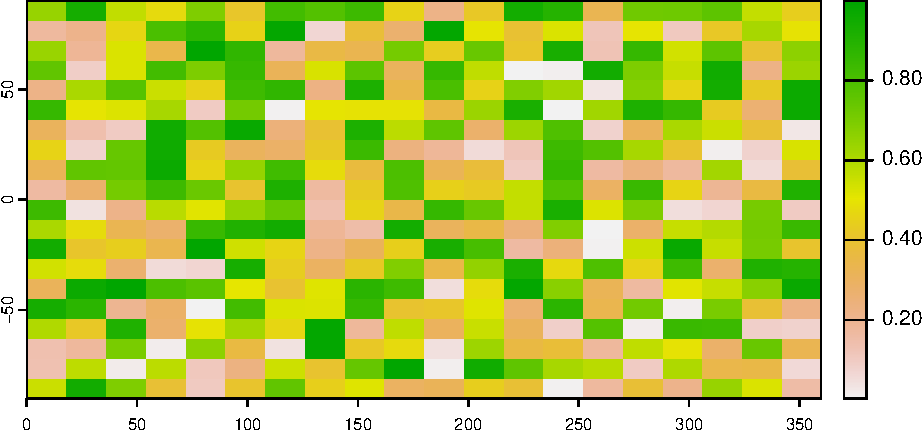
\includegraphics{R-spatial_files/figure-latex/unnamed-chunk-7-1.pdf}

(The \href{https://cran.r-project.org/web/packages/rasterVis/index.html}{\texttt{rasterVis} package} provides a set of methods for enhanced visualization and interaction for more advanced plotting of raster objects.)

\texttt{SpatRaster} objects can also be created from a matrix.

\begin{Shaded}
\begin{Highlighting}[]
\FunctionTok{class}\NormalTok{(volcano)}
\end{Highlighting}
\end{Shaded}

\begin{verbatim}
#> [1] "matrix" "array"
\end{verbatim}

\begin{Shaded}
\begin{Highlighting}[]
\NormalTok{volcano.r }\OtherTok{\textless{}{-}} \FunctionTok{rast}\NormalTok{(volcano)}
\FunctionTok{class}\NormalTok{(volcano.r)}
\end{Highlighting}
\end{Shaded}

\begin{verbatim}
#> [1] "SpatRaster"
#> attr(,"package")
#> [1] "terra"
\end{verbatim}

We also use the \texttt{rast()} function to read in a raster file. This raster is generated as part of the \href{https://www.neonscience.org/field-sites/field-sites-map/HARV}{NEON Harvard Forest field site}.

\begin{Shaded}
\begin{Highlighting}[]
\NormalTok{HARV }\OtherTok{\textless{}{-}} \FunctionTok{rast}\NormalTok{(}\StringTok{"data/HARV\_RGB\_Ortho.tif"}\NormalTok{)}
\end{Highlighting}
\end{Shaded}

Typing the name of the object will give us what's in there:

\begin{Shaded}
\begin{Highlighting}[]
\NormalTok{HARV}
\end{Highlighting}
\end{Shaded}

\begin{verbatim}
#> class       : SpatRaster 
#> dimensions  : 2317, 3073, 3  (nrow, ncol, nlyr)
#> resolution  : 0.25, 0.25  (x, y)
#> extent      : 731998.5, 732766.8, 4712956, 4713536  (xmin, xmax, ymin, ymax)
#> coord. ref. : WGS 84 / UTM zone 18N (EPSG:32618) 
#> source      : HARV_RGB_Ortho.tif 
#> names       : HARV_RGB_Ortho_1, HARV_RGB_Ortho_2, HARV_RGB_Ortho_3 
#> min values  :                0,                0,                0 
#> max values  :              255,              255,              255
\end{verbatim}

\begin{quote}
Challenge

Based on the output above answer the following questions:

\begin{enumerate}
\def\labelenumi{\arabic{enumi}.}
\tightlist
\item
  How many bands?
\item
  What are the names of the bands)?
\item
  Where are the cell values stored?
\item
  What is the CRS?
\end{enumerate}
\end{quote}

We can plot the object like this:

\begin{Shaded}
\begin{Highlighting}[]
\FunctionTok{plot}\NormalTok{(HARV)}
\end{Highlighting}
\end{Shaded}

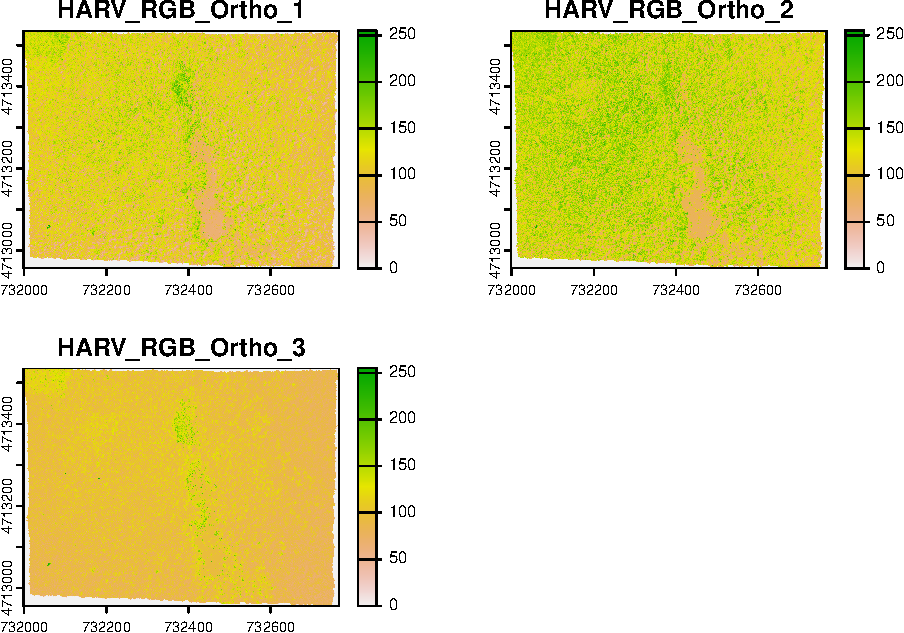
\includegraphics{R-spatial_files/figure-latex/plot-raster-1.pdf}

Or to plot a single band:

\begin{Shaded}
\begin{Highlighting}[]
\FunctionTok{plot}\NormalTok{(HARV, }\DecValTok{3}\NormalTok{)}
\end{Highlighting}
\end{Shaded}

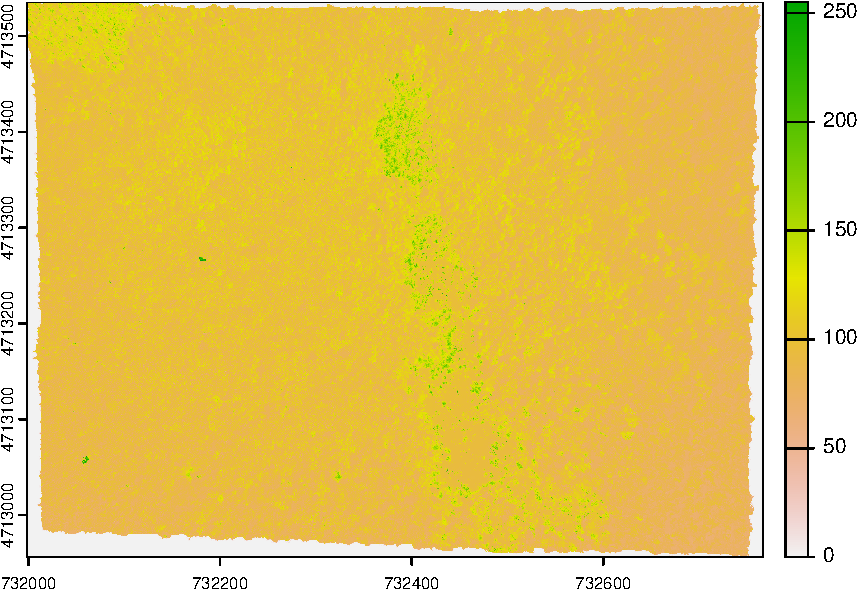
\includegraphics{R-spatial_files/figure-latex/plot-raster-single-1.pdf}

We can also use the \texttt{rast()} function to import one single band:

\begin{Shaded}
\begin{Highlighting}[]
\NormalTok{HARV\_Band2 }\OtherTok{\textless{}{-}} \FunctionTok{rast}\NormalTok{(}\StringTok{"data/HARV\_RGB\_Ortho.tif"}\NormalTok{, }\AttributeTok{lyrs =} \DecValTok{2}\NormalTok{)}
\FunctionTok{plot}\NormalTok{(HARV\_Band2)}
\end{Highlighting}
\end{Shaded}

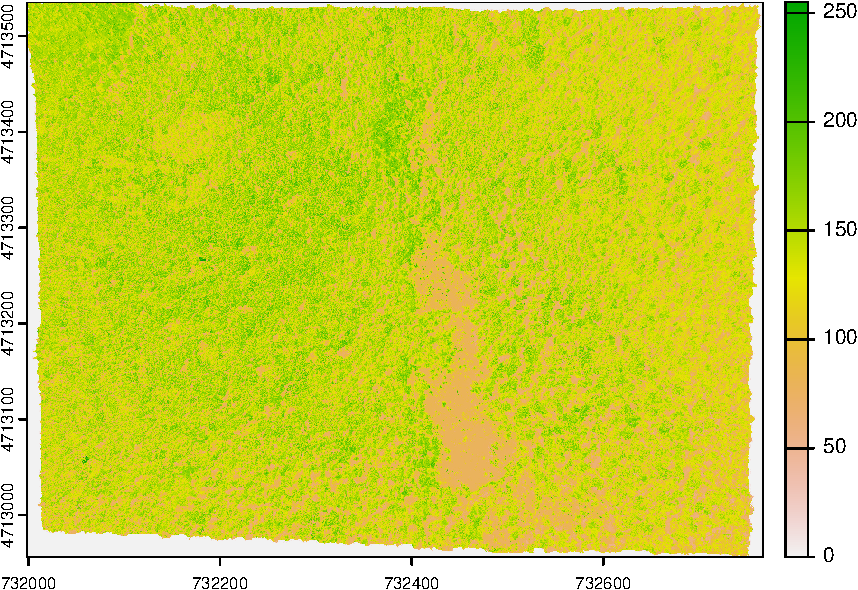
\includegraphics{R-spatial_files/figure-latex/one-multiband-1.pdf}

Let's now explore the distribution of values contained within our raster using the \texttt{hist()} function which produces a histogram. Histograms are often useful in identifying outliers and bad data values in our raster data.

\begin{Shaded}
\begin{Highlighting}[]
\FunctionTok{hist}\NormalTok{(HARV)}
\end{Highlighting}
\end{Shaded}

\begin{verbatim}
#> Warning: [hist] a sample of 14% of the cells was used

#> Warning: [hist] a sample of 14% of the cells was used

#> Warning: [hist] a sample of 14% of the cells was used
\end{verbatim}

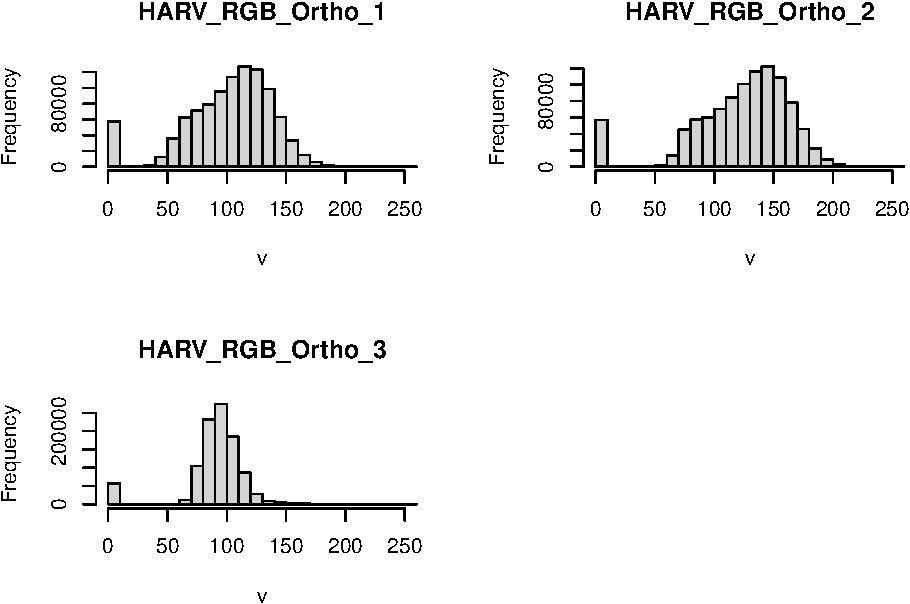
\includegraphics{R-spatial_files/figure-latex/n-hist-1.pdf}

Notice that a warning message is produced when R creates the histogram. By default the maximum cells processed per band is 1,000,000. This maximum value is to ensure processing efficiency as our data become larger. We can force the \texttt{hist} function to use all cell values.

\begin{Shaded}
\begin{Highlighting}[]
\FunctionTok{ncell}\NormalTok{(HARV)}
\end{Highlighting}
\end{Shaded}

\begin{verbatim}
#> [1] 7120141
\end{verbatim}

\begin{Shaded}
\begin{Highlighting}[]
\FunctionTok{hist}\NormalTok{(HARV, }\AttributeTok{maxcell =} \FunctionTok{ncell}\NormalTok{(HARV))}
\end{Highlighting}
\end{Shaded}

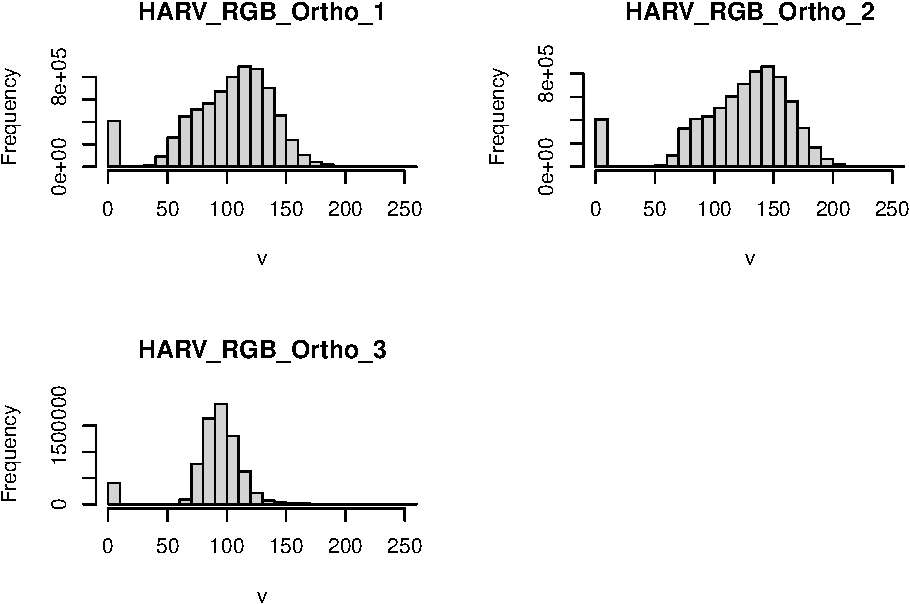
\includegraphics{R-spatial_files/figure-latex/n-hist-allvals-1.pdf}

At times it may be useful to explore raster metadata before loading them into R. This can be done with the function \texttt{describe()}

\begin{Shaded}
\begin{Highlighting}[]
\FunctionTok{describe}\NormalTok{(}\StringTok{"data/HARV\_RGB\_Ortho.tif"}\NormalTok{)}
\end{Highlighting}
\end{Shaded}

\begin{verbatim}
#>  [1] "Driver: GTiff/GeoTIFF"                                                                                                                                                                                                                                                          
#>  [2] "Files: data/HARV_RGB_Ortho.tif"                                                                                                                                                                                                                                                 
#>  [3] "Size is 3073, 2317"                                                                                                                                                                                                                                                             
#>  [4] "Coordinate System is:"                                                                                                                                                                                                                                                          
#>  [5] "PROJCRS[\"WGS 84 / UTM zone 18N\","                                                                                                                                                                                                                                             
#>  [6] "    BASEGEOGCRS[\"WGS 84\","                                                                                                                                                                                                                                                    
#>  [7] "        DATUM[\"World Geodetic System 1984\","                                                                                                                                                                                                                                  
#>  [8] "            ELLIPSOID[\"WGS 84\",6378137,298.257223563,"                                                                                                                                                                                                                        
#>  [9] "                LENGTHUNIT[\"metre\",1]]],"                                                                                                                                                                                                                                     
#> [10] "        PRIMEM[\"Greenwich\",0,"                                                                                                                                                                                                                                                
#> [11] "            ANGLEUNIT[\"degree\",0.0174532925199433]],"                                                                                                                                                                                                                         
#> [12] "        ID[\"EPSG\",4326]],"                                                                                                                                                                                                                                                    
#> [13] "    CONVERSION[\"UTM zone 18N\","                                                                                                                                                                                                                                               
#> [14] "        METHOD[\"Transverse Mercator\","                                                                                                                                                                                                                                        
#> [15] "            ID[\"EPSG\",9807]],"                                                                                                                                                                                                                                                
#> [16] "        PARAMETER[\"Latitude of natural origin\",0,"                                                                                                                                                                                                                            
#> [17] "            ANGLEUNIT[\"degree\",0.0174532925199433],"                                                                                                                                                                                                                          
#> [18] "            ID[\"EPSG\",8801]],"                                                                                                                                                                                                                                                
#> [19] "        PARAMETER[\"Longitude of natural origin\",-75,"                                                                                                                                                                                                                         
#> [20] "            ANGLEUNIT[\"degree\",0.0174532925199433],"                                                                                                                                                                                                                          
#> [21] "            ID[\"EPSG\",8802]],"                                                                                                                                                                                                                                                
#> [22] "        PARAMETER[\"Scale factor at natural origin\",0.9996,"                                                                                                                                                                                                                   
#> [23] "            SCALEUNIT[\"unity\",1],"                                                                                                                                                                                                                                            
#> [24] "            ID[\"EPSG\",8805]],"                                                                                                                                                                                                                                                
#> [25] "        PARAMETER[\"False easting\",500000,"                                                                                                                                                                                                                                    
#> [26] "            LENGTHUNIT[\"metre\",1],"                                                                                                                                                                                                                                           
#> [27] "            ID[\"EPSG\",8806]],"                                                                                                                                                                                                                                                
#> [28] "        PARAMETER[\"False northing\",0,"                                                                                                                                                                                                                                        
#> [29] "            LENGTHUNIT[\"metre\",1],"                                                                                                                                                                                                                                           
#> [30] "            ID[\"EPSG\",8807]]],"                                                                                                                                                                                                                                               
#> [31] "    CS[Cartesian,2],"                                                                                                                                                                                                                                                           
#> [32] "        AXIS[\"(E)\",east,"                                                                                                                                                                                                                                                     
#> [33] "            ORDER[1],"                                                                                                                                                                                                                                                          
#> [34] "            LENGTHUNIT[\"metre\",1]],"                                                                                                                                                                                                                                          
#> [35] "        AXIS[\"(N)\",north,"                                                                                                                                                                                                                                                    
#> [36] "            ORDER[2],"                                                                                                                                                                                                                                                          
#> [37] "            LENGTHUNIT[\"metre\",1]],"                                                                                                                                                                                                                                          
#> [38] "    USAGE["                                                                                                                                                                                                                                                                     
#> [39] "        SCOPE[\"Engineering survey, topographic mapping.\"],"                                                                                                                                                                                                                   
#> [40] "        AREA[\"Between 78°W and 72°W, northern hemisphere between equator and 84°N, onshore and offshore. Bahamas. Canada - Nunavut; Ontario; Quebec. Colombia. Cuba. Ecuador. Greenland. Haiti. Jamaica. Panama. Turks and Caicos Islands. United States (USA). Venezuela.\"],"
#> [41] "        BBOX[0,-78,84,-72]],"                                                                                                                                                                                                                                                   
#> [42] "    ID[\"EPSG\",32618]]"                                                                                                                                                                                                                                                        
#> [43] "Data axis to CRS axis mapping: 1,2"                                                                                                                                                                                                                                             
#> [44] "Origin = (731998.500000000000000,4713535.500000000000000)"                                                                                                                                                                                                                      
#> [45] "Pixel Size = (0.250000000000000,-0.250000000000000)"                                                                                                                                                                                                                            
#> [46] "Metadata:"                                                                                                                                                                                                                                                                      
#> [47] "  AREA_OR_POINT=Area"                                                                                                                                                                                                                                                           
#> [48] "Image Structure Metadata:"                                                                                                                                                                                                                                                      
#> [49] "  COMPRESSION=LZW"                                                                                                                                                                                                                                                              
#> [50] "  INTERLEAVE=PIXEL"                                                                                                                                                                                                                                                             
#> [51] "Corner Coordinates:"                                                                                                                                                                                                                                                            
#> [52] "Upper Left  (  731998.500, 4713535.500) ( 72d10'29.27\"W, 42d32'21.80\"N)"                                                                                                                                                                                                      
#> [53] "Lower Left  (  731998.500, 4712956.250) ( 72d10'30.11\"W, 42d32' 3.04\"N)"                                                                                                                                                                                                      
#> [54] "Upper Right (  732766.750, 4713535.500) ( 72d 9'55.63\"W, 42d32'20.97\"N)"                                                                                                                                                                                                      
#> [55] "Lower Right (  732766.750, 4712956.250) ( 72d 9'56.48\"W, 42d32' 2.21\"N)"                                                                                                                                                                                                      
#> [56] "Center      (  732382.625, 4713245.875) ( 72d10'12.87\"W, 42d32'12.00\"N)"                                                                                                                                                                                                      
#> [57] "Band 1 Block=3073x1 Type=Float64, ColorInterp=Gray"                                                                                                                                                                                                                             
#> [58] "  Min=0.000 Max=255.000 "                                                                                                                                                                                                                                                       
#> [59] "  Minimum=0.000, Maximum=255.000, Mean=nan, StdDev=nan"                                                                                                                                                                                                                         
#> [60] "  NoData Value=-1.7e+308"                                                                                                                                                                                                                                                       
#> [61] "  Metadata:"                                                                                                                                                                                                                                                                    
#> [62] "    STATISTICS_MAXIMUM=255"                                                                                                                                                                                                                                                     
#> [63] "    STATISTICS_MEAN=nan"                                                                                                                                                                                                                                                        
#> [64] "    STATISTICS_MINIMUM=0"                                                                                                                                                                                                                                                       
#> [65] "    STATISTICS_STDDEV=nan"                                                                                                                                                                                                                                                      
#> [66] "Band 2 Block=3073x1 Type=Float64, ColorInterp=Undefined"                                                                                                                                                                                                                        
#> [67] "  Min=0.000 Max=255.000 "                                                                                                                                                                                                                                                       
#> [68] "  Minimum=0.000, Maximum=255.000, Mean=nan, StdDev=nan"                                                                                                                                                                                                                         
#> [69] "  NoData Value=-1.7e+308"                                                                                                                                                                                                                                                       
#> [70] "  Metadata:"                                                                                                                                                                                                                                                                    
#> [71] "    STATISTICS_MAXIMUM=255"                                                                                                                                                                                                                                                     
#> [72] "    STATISTICS_MEAN=nan"                                                                                                                                                                                                                                                        
#> [73] "    STATISTICS_MINIMUM=0"                                                                                                                                                                                                                                                       
#> [74] "    STATISTICS_STDDEV=nan"                                                                                                                                                                                                                                                      
#> [75] "Band 3 Block=3073x1 Type=Float64, ColorInterp=Undefined"                                                                                                                                                                                                                        
#> [76] "  Min=0.000 Max=255.000 "                                                                                                                                                                                                                                                       
#> [77] "  Minimum=0.000, Maximum=255.000, Mean=nan, StdDev=nan"                                                                                                                                                                                                                         
#> [78] "  NoData Value=-1.7e+308"                                                                                                                                                                                                                                                       
#> [79] "  Metadata:"                                                                                                                                                                                                                                                                    
#> [80] "    STATISTICS_MAXIMUM=255"                                                                                                                                                                                                                                                     
#> [81] "    STATISTICS_MEAN=nan"                                                                                                                                                                                                                                                        
#> [82] "    STATISTICS_MINIMUM=0"                                                                                                                                                                                                                                                       
#> [83] "    STATISTICS_STDDEV=nan"
\end{verbatim}

For the many functions available for working with such an object see:

\begin{Shaded}
\begin{Highlighting}[]
\FunctionTok{methods}\NormalTok{(}\AttributeTok{class=}\StringTok{"SpatRaster"}\NormalTok{)}
\end{Highlighting}
\end{Shaded}

\begin{verbatim}
#>   [1] !                     [                     [[                   
#>   [4] [[<-                  [<-                   %in%                 
#>   [7] $                     $<-                   activeCat            
#>  [10] activeCat<-           add<-                 addCats              
#>  [13] adjacent              aggregate             align                
#>  [16] all.equal             allNA                 animate              
#>  [19] anyNA                 app                   approximate          
#>  [22] area                  Arith                 as.array             
#>  [25] as.bool               as.character          as.contour           
#>  [28] as.data.frame         as.factor             as.int               
#>  [31] as.integer            as.lines              as.list              
#>  [34] as.logical            as.matrix             as.numeric           
#>  [37] as.points             as.polygons           as.raster            
#>  [40] atan_2                atan2                 autocor              
#>  [43] barplot               blocks                boundaries           
#>  [46] boxplot               buffer                c                    
#>  [49] catalyze              categories            cats                 
#>  [52] cellFromRowCol        cellFromRowColCombine cellFromXY           
#>  [55] cells                 cellSize              clamp_ts             
#>  [58] clamp                 classify              click                
#>  [61] coerce                colFromCell           colFromX             
#>  [64] colorize              coltab                coltab<-             
#>  [67] Compare               compare               compareGeom          
#>  [70] concats               contour               costDist             
#>  [73] countNA               cover                 crds                 
#>  [76] crop                  crosstab              crs                  
#>  [79] crs<-                 datatype              deepcopy             
#>  [82] density               depth                 depth<-              
#>  [85] diff                  dim                   dim<-                
#>  [88] direction             disagg                distance             
#>  [91] droplevels            expanse               ext                  
#>  [94] ext<-                 extend                extract              
#>  [97] extractRange          fillTime              flip                 
#> [100] focal                 focal3D               focalCor             
#> [103] focalCpp              focalPairs            focalReg             
#> [106] focalValues           freq                  getTileExtents       
#> [109] global                gridDist              gridDistance         
#> [112] has.colors            has.RGB               has.time             
#> [115] hasMinMax             hasValues             head                 
#> [118] hist                  identical             ifel                 
#> [121] image                 init                  inMemory             
#> [124] inset                 interpIDW             interpNear           
#> [127] interpolate           intersect             is.bool              
#> [130] is.factor             is.finite             is.infinite          
#> [133] is.int                is.lonlat             is.na                
#> [136] is.nan                is.related            is.rotated           
#> [139] isFALSE               isTRUE                k_means              
#> [142] lapp                  layerCor              levels               
#> [145] levels<-              linearUnits           lines                
#> [148] log                   Logic                 logic                
#> [151] longnames             longnames<-           makeTiles            
#> [154] mask                  match                 math                 
#> [157] Math                  Math2                 mean                 
#> [160] median                merge                 meta                 
#> [163] metags                metags<-              minmax               
#> [166] modal                 mosaic                NAflag               
#> [169] NAflag<-              names                 names<-              
#> [172] ncell                 ncol                  ncol<-               
#> [175] nlyr                  nlyr<-                noNA                 
#> [178] not.na                nrow                  nrow<-               
#> [181] nsrc                  origin                origin<-             
#> [184] pairs                 panel                 patches              
#> [187] persp                 plet                  plot                 
#> [190] plotRGB               points                polys                
#> [193] prcomp                predict               princomp             
#> [196] project               quantile              rangeFill            
#> [199] rapp                  rast                  rasterize            
#> [202] rasterizeGeom         rasterizeWin          rcl                  
#> [205] readStart             readStop              readValues           
#> [208] rectify               regress               relate               
#> [211] rep                   res                   res<-                
#> [214] resample              rescale               rev                  
#> [217] RGB                   RGB<-                 roll                 
#> [220] rotate                rowColCombine         rowColFromCell       
#> [223] rowFromCell           rowFromY              sapp                 
#> [226] saveRDS               scale                 scoff                
#> [229] scoff<-               sds                   segregate            
#> [232] sel                   selectHighest         selectRange          
#> [235] serialize             set.cats              set.crs              
#> [238] set.ext               set.names             set.RGB              
#> [241] set.values            setMinMax             setValues            
#> [244] shift                 show                  sieve                
#> [247] size                  sort                  sources              
#> [250] spatSample            split                 sprc                 
#> [253] st_bbox               st_crs                stdev                
#> [256] str                   stretch               subset               
#> [259] subst                 summary               Summary              
#> [262] t                     tail                  tapp                 
#> [265] terrain               text                  tighten              
#> [268] time                  time<-                timeInfo             
#> [271] trans                 trim                  unique               
#> [274] units                 units<-               update               
#> [277] values                values<-              varnames             
#> [280] varnames<-            viewshed              weighted.mean        
#> [283] where.max             where.min             which.lyr            
#> [286] which.max             which.min             window               
#> [289] window<-              wrap                  wrapCache            
#> [292] writeCDF              writeRaster           writeStart           
#> [295] writeStop             writeValues           xapp                 
#> [298] xFromCell             xFromCol              xmax                 
#> [301] xmax<-                xmin                  xmin<-               
#> [304] xres                  xyFromCell            yFromCell            
#> [307] yFromRow              ymax                  ymax<-               
#> [310] ymin                  ymin<-                yres                 
#> [313] zonal                 zoom                 
#> see '?methods' for accessing help and source code
\end{verbatim}

\hypertarget{spatialops}{%
\chapter{Spatial data manipulation in R}\label{spatialops}}

\begin{quote}
Learning Objectives

\begin{itemize}
\tightlist
\item
  Join attribute data to a polygon vector file
\item
  Reproject a vector file
\item
  Select polygons of a vector by location
\item
  Reproject a raster
\item
  Perform a raster calculation
\end{itemize}
\end{quote}

\begin{center}\rule{0.5\linewidth}{0.5pt}\end{center}

There are a wide variety of spatial, topological, and attribute data operations you can perform with R. \href{https://r.geocompx.org/}{Lovelace et al's recent publication}\footnote{Lovelace, R., Nowosad, J., \& Muenchow, J. (2024). Geocomputation with R. CRC Press.} goes into great depth about this and is highly recommended.

In this section we will look at a few examples for libraries and commands that allow us to process spatial data in R and perform a few commonly used operations.

\hypertarget{attribute-join}{%
\section{Attribute Join}\label{attribute-join}}

An attribute join on vector data brings tabular data into a geographic context. It refers to the process of joining data in tabular format to data in a format that holds the geometries (polygon, line, or point).

If you have done attribute joins of shapefiles in GIS software like \emph{ArcGIS} or \emph{QGis} you know that you need a \textbf{unique identifier} in both the attribute table of the shapefile and the table to be joined.

First we will load the CSV table \texttt{PhiladelphiaEduAttain.csv} into a dataframe in R and name it \texttt{ph\_edu}.

\begin{Shaded}
\begin{Highlighting}[]
\NormalTok{ph\_edu }\OtherTok{\textless{}{-}} \FunctionTok{read\_csv}\NormalTok{(}\StringTok{"data/PhiladelphiaEduAttain.csv"}\NormalTok{)}
\end{Highlighting}
\end{Shaded}

\begin{verbatim}
#> Rows: 384 Columns: 13
#> -- Column specification --------------------------------------------------------
#> Delimiter: ","
#> chr  (1): NAME
#> dbl (12): GEOID, fem_bachelor, fem_doctorate, fem_highschool, fem_noschool, ...
#> 
#> i Use `spec()` to retrieve the full column specification for this data.
#> i Specify the column types or set `show_col_types = FALSE` to quiet this message.
\end{verbatim}

\begin{Shaded}
\begin{Highlighting}[]
\FunctionTok{names}\NormalTok{(ph\_edu)}
\end{Highlighting}
\end{Shaded}

If you don't have the object still loaded read the the \texttt{PhillyTotalPopHHinc} shapefile into an object named \texttt{philly\_sf}. Check out the column names of \texttt{philly\_sf} and of \texttt{ph\_edu} to determine which one might contain the unique identifier for the join.

\begin{Shaded}
\begin{Highlighting}[]
\CommentTok{\# if you need to read in again:}
\CommentTok{\# philly\_sf \textless{}{-} st\_read("data/Philly/")}
\FunctionTok{names}\NormalTok{(philly\_sf)}
\end{Highlighting}
\end{Shaded}

To join the \texttt{ph\_edu} data frame with \texttt{philly\_sf} we can use \texttt{merge} like this:

\begin{Shaded}
\begin{Highlighting}[]
\NormalTok{philly\_sf\_merged }\OtherTok{\textless{}{-}} \FunctionTok{left\_join}\NormalTok{(philly\_sf, ph\_edu, }\AttributeTok{by =} \FunctionTok{c}\NormalTok{(}\StringTok{"GEOID10"} \OtherTok{=} \StringTok{"GEOID"}\NormalTok{))}
\FunctionTok{names}\NormalTok{(philly\_sf\_merged) }
\end{Highlighting}
\end{Shaded}

\begin{verbatim}
#>  [1] "STATEFP10"       "COUNTYFP10"      "TRACTCE10"       "GEOID10"        
#>  [5] "NAME10"          "NAMELSAD10"      "MTFCC10"         "FUNCSTAT10"     
#>  [9] "ALAND10"         "AWATER10"        "INTPTLAT10"      "INTPTLON10"     
#> [13] "GISJOIN"         "Shape_area"      "Shape_len"       "medHHinc"       
#> [17] "totalPop"        "NAME"            "fem_bachelor"    "fem_doctorate"  
#> [21] "fem_highschool"  "fem_noschool"    "fem_ovr_25"      "male_bachelor"  
#> [25] "male_doctorate"  "male_highschool" "male_noschool"   "male_ovr_25"    
#> [29] "pop_ovr_25"      "geometry"
\end{verbatim}

We see the new attribute columns added, as well as the geometry column.

\hypertarget{topological-subsetting-select-polygons-by-location}{%
\section{Topological Subsetting: Select Polygons by Location}\label{topological-subsetting-select-polygons-by-location}}

For the next example our goal is to select all Philadelphia census tracts within a range of 2 kilometers from the city center.

\begin{quote}
Think about this for a moment -- what might be the steps you'd follow?
\end{quote}

\begin{Shaded}
\begin{Highlighting}[]
\DocumentationTok{\#\# How about:}

\CommentTok{\# 1. Get the census tract polygons.}
\CommentTok{\# 2. Find the Philadelphia city center coordinates.}
\CommentTok{\# 3. Create a buffer around the city center point.}
\CommentTok{\# 4. Select all census tract polygons that intersect with the center buffer}
\end{Highlighting}
\end{Shaded}

We will use \texttt{philly\_sf} for the census tract polygons.

In addition, we need to create a \texttt{sf} Point object with the Philadelphia city center coordinates:

\[x = 1750160\]
\[y = 467499.9\]

These coordinates are also in the \emph{USA Contiguous Albers Equal Area Conic} projected CRS, which is the same as CRS as \texttt{philly\_sf}.

With this information, we create a object that holds the coordinates of the city center. Since we don't have attributes we will just create it as a simple feature collection, \texttt{scf}.

\begin{Shaded}
\begin{Highlighting}[]
\CommentTok{\# if you need to read in again:}
\CommentTok{\# philly\_sf \textless{}{-} st\_read("data/Philly/", quiet = T)}

\CommentTok{\# make a simple feature point with CRS}
\NormalTok{philly\_ctr\_sfc }\OtherTok{\textless{}{-}} \FunctionTok{st\_sfc}\NormalTok{(}\FunctionTok{st\_point}\NormalTok{(}\FunctionTok{c}\NormalTok{(}\DecValTok{1750160}\NormalTok{, }\FloatTok{467499.9}\NormalTok{)), }\AttributeTok{crs =} \FunctionTok{st\_crs}\NormalTok{(philly\_sf))}
\end{Highlighting}
\end{Shaded}

For the spatial operations we can recur to the suite of geometric operations that come with the \texttt{sf} package.

We create a 2km buffer around the city center point:

\begin{Shaded}
\begin{Highlighting}[]
\NormalTok{philly\_buf }\OtherTok{\textless{}{-}} \FunctionTok{st\_buffer}\NormalTok{(philly\_ctr\_sfc, }\DecValTok{2000}\NormalTok{)}
\end{Highlighting}
\end{Shaded}

Ok. Now we can use that buffer to select all census tract polygons that intersect with the center buffer. In order to determine the polygons we use \texttt{st\_intersects}, a geometric binary which returns a vector of indices of the polygons that intersect with the buffer.

\begin{Shaded}
\begin{Highlighting}[]
\NormalTok{philly\_intersects }\OtherTok{\textless{}{-}} \FunctionTok{st\_intersects}\NormalTok{(philly\_buf, philly\_sf)}
\NormalTok{philly\_intersects}
\end{Highlighting}
\end{Shaded}

\begin{verbatim}
#> Sparse geometry binary predicate list of length 1, where the predicate
#> was `intersects'
#>  1: 3, 10, 11, 12, 13, 19, 20, 21, 50, 51, ...
\end{verbatim}

We have created a \texttt{sgbp} object, which is a ``Sparse Geometry Binary Predicate''. It is a so called sparse matrix, which is a list with integer vectors only holding the indices for each polygon that intersects. In our case we only have one vector, because we only intersect with one buffer polygon, so we can extract this first vector with \texttt{philly\_buf\_intersects{[}{[}1{]}{]}} and use it for subsetting:

\begin{Shaded}
\begin{Highlighting}[]
\NormalTok{philly\_sel}\OtherTok{\textless{}{-}}\NormalTok{ philly\_sf[philly\_intersects[[}\DecValTok{1}\NormalTok{]],]}

\CommentTok{\# plot}
\FunctionTok{plot}\NormalTok{(}\FunctionTok{st\_geometry}\NormalTok{(philly\_sf), }\AttributeTok{border=}\StringTok{"\#aaaaaa"}\NormalTok{, }\AttributeTok{main=}\StringTok{"Census tracts that overlap with 2km buffer around city center"}\NormalTok{)}
\FunctionTok{plot}\NormalTok{(}\FunctionTok{st\_geometry}\NormalTok{(philly\_sel), }\AttributeTok{add=}\NormalTok{T, }\AttributeTok{col=}\StringTok{"red"}\NormalTok{)}
\FunctionTok{plot}\NormalTok{(}\FunctionTok{st\_geometry}\NormalTok{(philly\_buf), }\AttributeTok{add=}\NormalTok{T, }\AttributeTok{lwd =} \DecValTok{2}\NormalTok{)}
\end{Highlighting}
\end{Shaded}

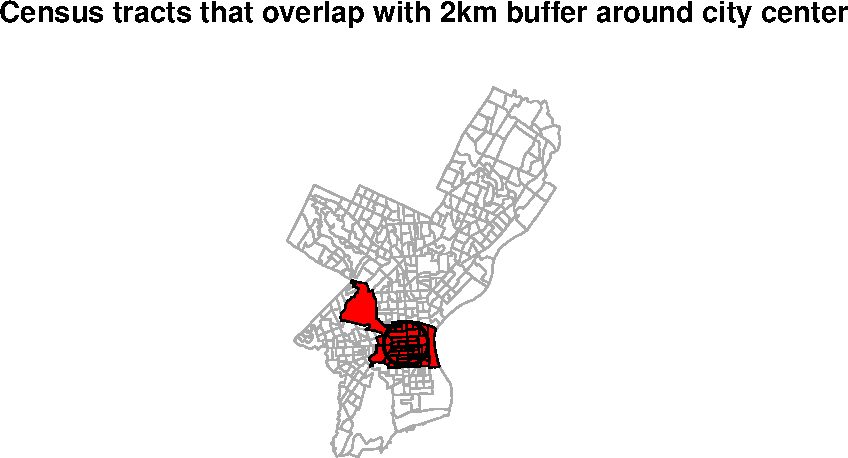
\includegraphics{R-spatial_files/figure-latex/sf-intersects-subset-1.pdf}

Note the difference to \texttt{st\_intersection}, which performs a geometric operation and creates a new sf object which cuts out the area of the buffer from the polygons like cookie a cutter:

\begin{Shaded}
\begin{Highlighting}[]
\NormalTok{philly\_intersection }\OtherTok{\textless{}{-}} \FunctionTok{st\_intersection}\NormalTok{(philly\_buf, philly\_sf)}
\NormalTok{philly\_intersection}
\end{Highlighting}
\end{Shaded}

\begin{verbatim}
#> Geometry set for 46 features 
#> Geometry type: GEOMETRY
#> Dimension:     XY
#> Bounding box:  xmin: 1748160 ymin: 465499.9 xmax: 1752160 ymax: 469499.9
#> Projected CRS: Albers
#> First 5 geometries:
\end{verbatim}

\begin{verbatim}
#> POLYGON ((1752157 467395.2, 1752153 467339.7, 1...
\end{verbatim}

\begin{verbatim}
#> POLYGON ((1752149 467290.8, 1752135 467187, 175...
\end{verbatim}

\begin{verbatim}
#> POLYGON ((1751347 466573.5, 1751321 467037.6, 1...
\end{verbatim}

\begin{verbatim}
#> POLYGON ((1750298 467616.7, 1750148 467615.2, 1...
\end{verbatim}

\begin{verbatim}
#> POLYGON ((1748853 467255, 1748874 467605.3, 174...
\end{verbatim}

\begin{Shaded}
\begin{Highlighting}[]
\FunctionTok{plot}\NormalTok{(}\FunctionTok{st\_geometry}\NormalTok{(philly\_sf), }\AttributeTok{border=}\StringTok{"\#aaaaaa"}\NormalTok{, }\AttributeTok{main=}\StringTok{"Census tracts around city center, clipped by 2km buffer "}\NormalTok{)}
\FunctionTok{plot}\NormalTok{(philly\_intersection, }\AttributeTok{add=}\NormalTok{T, }\AttributeTok{lwd =} \DecValTok{2}\NormalTok{, }\AttributeTok{border =} \StringTok{"red"}\NormalTok{)}
\end{Highlighting}
\end{Shaded}

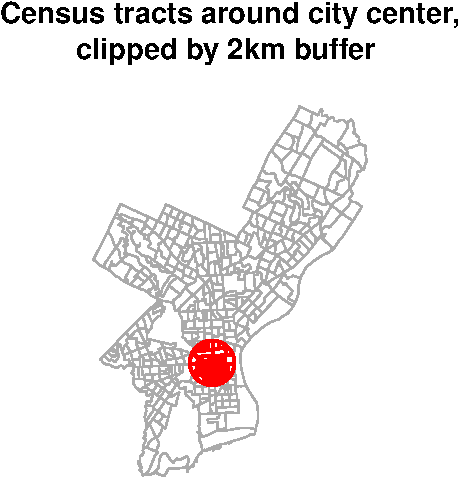
\includegraphics{R-spatial_files/figure-latex/sf-intersection-1.pdf}

\hypertarget{reprojecting}{%
\section{Reprojecting}\label{reprojecting}}

Occasionally you may have to change the coordinates of your spatial object into a new Coordinate Reference System (CRS). Functions to transform, or \emph{reproject} spatial objects typically take the following two arguments:

\begin{itemize}
\tightlist
\item
  the spatial object to reproject
\item
  a CRS object with the new projection definition
\end{itemize}

You can reproject

\begin{itemize}
\tightlist
\item
  a \texttt{sf} object with \texttt{st\_transform()}\\
\item
  a \texttt{SpatRaster} object with \texttt{project()}
\end{itemize}

The perhaps trickiest part here is to determine the definition of the projection, which needs to be a character string in \href{http://trac.osgeo.org/proj/}{proj4} format. You can \href{http://www.spatialreference.org}{look it up online}. For example for \href{http://spatialreference.org/ref/epsg/wgs-84-utm-zone-33n/}{UTM zone 33N (EPSG:32633)} the string would be:

\href{http://spatialreference.org/ref/epsg/wgs-84-utm-zone-33n/proj4js/}{\texttt{+proj=utm\ +zone=33\ +ellps=WGS84\ +datum=WGS84\ +units=m\ +no\_defs}}

You can retrieve the CRS:

\begin{itemize}
\tightlist
\item
  from an \texttt{sf} object with \texttt{st\_crs()}
\item
  from a \texttt{SpatRaster} object with \texttt{crs()}
\end{itemize}

Let us go back to the \texttt{"PhillyHomicides"} shapefile we exported earlier. Let's read it back in and reproject it so it matches the projection of the Philadelphia Census tracts.

Now let us check the CRS for both files.

\begin{Shaded}
\begin{Highlighting}[]
\CommentTok{\#If you need to read the file back in:}
\CommentTok{\#philly\_homicides\_sf \textless{}{-} st\_read("data/PhillyHomicides/")}

\FunctionTok{st\_crs}\NormalTok{(philly\_sf)}\SpecialCharTok{$}\NormalTok{proj4string}
\end{Highlighting}
\end{Shaded}

\begin{verbatim}
#> [1] "+proj=aea +lat_0=37.5 +lon_0=-96 +lat_1=29.5 +lat_2=45.5 +x_0=0 +y_0=0 +ellps=GRS80 +units=m +no_defs"
\end{verbatim}

\begin{Shaded}
\begin{Highlighting}[]
\FunctionTok{st\_crs}\NormalTok{(philly\_homicides\_sf)}\SpecialCharTok{$}\NormalTok{proj4string}
\end{Highlighting}
\end{Shaded}

\begin{verbatim}
#> [1] "+proj=longlat +datum=WGS84 +no_defs"
\end{verbatim}

We see that the CRS are different: we have \texttt{+proj=aea...} and \texttt{+proj=longlat...}. AEA refers to \emph{USA Contiguous Albers Equal Area Conic} which is a projected coordinate system with numeric units. We will need this below for our spatial operations, so we will make sure both files are in that same CRS.

We use \texttt{st\_transform} and assign the result to a new object. Note how we also use \texttt{str\_crs} to extract the projection definition from \texttt{philly\_sf}, so we don't have to type it out.

\begin{Shaded}
\begin{Highlighting}[]
\NormalTok{philly\_homicides\_sf\_aea }\OtherTok{\textless{}{-}} \FunctionTok{st\_transform}\NormalTok{(philly\_homicides\_sf, }\FunctionTok{st\_crs}\NormalTok{(philly\_sf))}
\end{Highlighting}
\end{Shaded}

We can use the \texttt{range()} command from the R base package to compare the coordinates before and after reprojection and confirm that we actually have transformed them. \texttt{range()} returns the \emph{min} and \emph{max} value of a vector of numbers.

\begin{Shaded}
\begin{Highlighting}[]
\FunctionTok{range}\NormalTok{(}\FunctionTok{st\_coordinates}\NormalTok{(philly\_homicides\_sf))}
\end{Highlighting}
\end{Shaded}

\begin{verbatim}
#> [1] -75.26809  40.13086
\end{verbatim}

\begin{Shaded}
\begin{Highlighting}[]
\FunctionTok{range}\NormalTok{(}\FunctionTok{st\_coordinates}\NormalTok{(philly\_homicides\_sf\_aea))}
\end{Highlighting}
\end{Shaded}

\begin{verbatim}
#> [1]  457489.7 1763671.8
\end{verbatim}

We can also compare them visually with:

\begin{Shaded}
\begin{Highlighting}[]
\FunctionTok{par}\NormalTok{(}\AttributeTok{mfrow=}\FunctionTok{c}\NormalTok{(}\DecValTok{1}\NormalTok{,}\DecValTok{2}\NormalTok{)) }
\FunctionTok{plot}\NormalTok{(}\FunctionTok{st\_geometry}\NormalTok{(philly\_homicides\_sf), }\AttributeTok{axes=}\ConstantTok{TRUE}\NormalTok{, }\AttributeTok{main =} \StringTok{"before transform {-} latlon"}\NormalTok{)}
\FunctionTok{plot}\NormalTok{(}\FunctionTok{st\_geometry}\NormalTok{(philly\_homicides\_sf\_aea), }\AttributeTok{axes=}\ConstantTok{TRUE}\NormalTok{, }\AttributeTok{main =} \StringTok{"after transform {-} aea"}\NormalTok{)}
\end{Highlighting}
\end{Shaded}

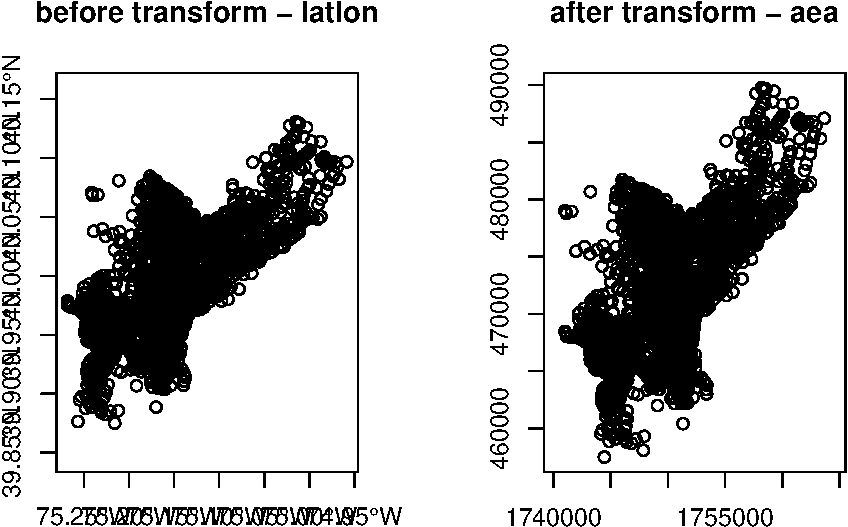
\includegraphics{R-spatial_files/figure-latex/compare-reproj-plots-sf-1.pdf}

Lastly, let us save the reprojected file as \texttt{PhillyHomicides\_aea} shapefile, as we will use it later on.

\begin{Shaded}
\begin{Highlighting}[]
\FunctionTok{st\_write}\NormalTok{(philly\_homicides\_sf\_aea, }\StringTok{"data/PhillyHomicides\_aea"}\NormalTok{, }\AttributeTok{driver =} \StringTok{"ESRI Shapefile"}\NormalTok{)}
\end{Highlighting}
\end{Shaded}

\hypertarget{raster-reprojection}{%
\subsection{Raster reprojection}\label{raster-reprojection}}

Here is what it would look like to reproject the HARV raster used earlier to a WGS84 projection. We see that see that the original projection is in UTM.

\begin{Shaded}
\begin{Highlighting}[]
\CommentTok{\# if you need to load again:}
\CommentTok{\#HARV \textless{}{-} raster("data/HARV\_RGB\_Ortho.tif")}
\FunctionTok{crs}\NormalTok{(HARV, }\AttributeTok{proj =} \ConstantTok{TRUE}\NormalTok{)}
\end{Highlighting}
\end{Shaded}

\begin{verbatim}
#> [1] "+proj=utm +zone=18 +datum=WGS84 +units=m +no_defs"
\end{verbatim}

\begin{Shaded}
\begin{Highlighting}[]
\NormalTok{HARV\_WGS84 }\OtherTok{\textless{}{-}} \FunctionTok{project}\NormalTok{(HARV, }\StringTok{"+init=epsg:4326"}\NormalTok{)}
\FunctionTok{crs}\NormalTok{(HARV\_WGS84, }\AttributeTok{proj =} \ConstantTok{TRUE}\NormalTok{)}
\end{Highlighting}
\end{Shaded}

\begin{verbatim}
#> [1] "+proj=longlat +datum=WGS84 +no_defs"
\end{verbatim}

Let's look at the coordinates to see the effect:

\begin{Shaded}
\begin{Highlighting}[]
\FunctionTok{ext}\NormalTok{(HARV)}
\end{Highlighting}
\end{Shaded}

\begin{verbatim}
#> SpatExtent : 731998.5, 732766.75, 4712956.25, 4713535.5 (xmin, xmax, ymin, ymax)
\end{verbatim}

\begin{Shaded}
\begin{Highlighting}[]
\FunctionTok{ext}\NormalTok{(HARV\_WGS84)}
\end{Highlighting}
\end{Shaded}

\begin{verbatim}
#> SpatExtent : -72.1750316832584, -72.1654516638594, 42.5339461813323, 42.5393881837189 (xmin, xmax, ymin, ymax)
\end{verbatim}

Due to the reprojection the number of cells has also changed:

\begin{Shaded}
\begin{Highlighting}[]
\FunctionTok{ncell}\NormalTok{(HARV)}
\end{Highlighting}
\end{Shaded}

\begin{verbatim}
#> [1] 7120141
\end{verbatim}

\begin{Shaded}
\begin{Highlighting}[]
\FunctionTok{ncell}\NormalTok{(HARV\_WGS84)}
\end{Highlighting}
\end{Shaded}

\begin{verbatim}
#> [1] 6859650
\end{verbatim}

And here is the visual proof:

\begin{Shaded}
\begin{Highlighting}[]
\FunctionTok{plot}\NormalTok{(HARV, }\AttributeTok{main =} \StringTok{"before transform {-} UTM"}\NormalTok{)}
\end{Highlighting}
\end{Shaded}

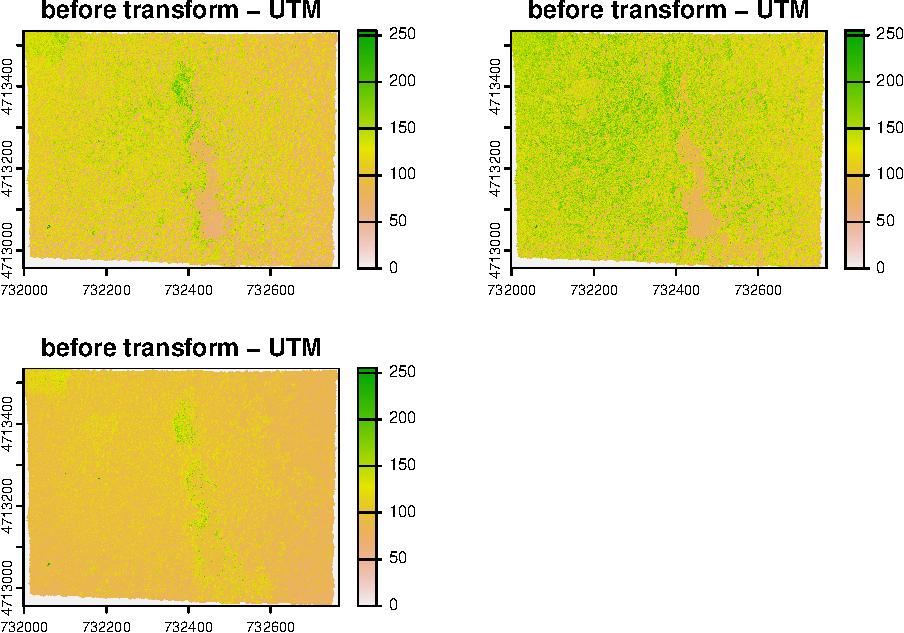
\includegraphics{R-spatial_files/figure-latex/raster-reproject-plot1-1.pdf}

\begin{Shaded}
\begin{Highlighting}[]
\FunctionTok{plot}\NormalTok{(HARV\_WGS84, }\AttributeTok{main =} \StringTok{"after transform {-} WGS84"}\NormalTok{)}
\end{Highlighting}
\end{Shaded}

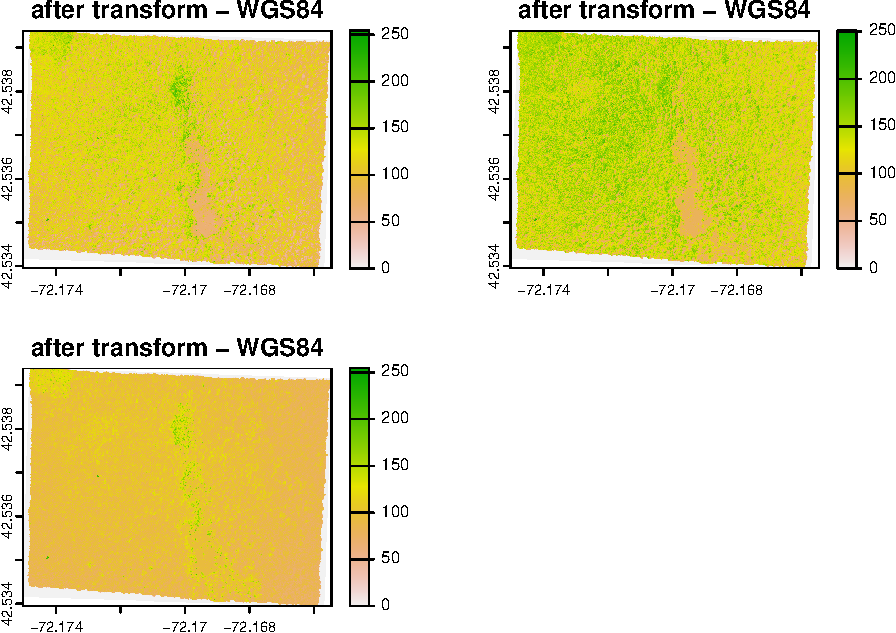
\includegraphics{R-spatial_files/figure-latex/raster-reproject-plot2-1.pdf}

\hypertarget{spatial-aggregation-points-in-polygons}{%
\section{Spatial Aggregation: Points in Polygons}\label{spatial-aggregation-points-in-polygons}}

Now that we have both homicides and census tracts in the same projection we will forge ahead and ask for the density of homicides for \textbf{each census tract} in Philadelphia: \(\frac{{homicides}}{area}\)

To achieve this this we join the points of homicide incidence to the census tract polygon and count them up for each polygon. You might be familiar with this operation from other GIS packages.

We will use piping and build up our object in the following way. First we calculate the area for each tract. We use the \texttt{st\_area} function on the geometry column and add the result.

\begin{Shaded}
\begin{Highlighting}[]
\NormalTok{philly\_sf }\SpecialCharTok{\%\textgreater{}\%} 
  \FunctionTok{mutate}\NormalTok{(}\AttributeTok{tract\_area =} \FunctionTok{st\_area}\NormalTok{(geometry)) }\SpecialCharTok{\%\textgreater{}\%} 
  \FunctionTok{head}\NormalTok{()}
\end{Highlighting}
\end{Shaded}

Next, we use st\_join to perform a spatial join with the points:

\begin{Shaded}
\begin{Highlighting}[]
\NormalTok{philly\_sf }\SpecialCharTok{\%\textgreater{}\%} 
  \FunctionTok{mutate}\NormalTok{(}\AttributeTok{tract\_area =} \FunctionTok{st\_area}\NormalTok{(geometry)) }\SpecialCharTok{\%\textgreater{}\%} 
  \FunctionTok{st\_join}\NormalTok{(philly\_homicides\_sf\_aea) }\SpecialCharTok{\%\textgreater{}\%}
  \FunctionTok{head}\NormalTok{()}
\end{Highlighting}
\end{Shaded}

Now we can group by a variable that uiquely identifies the census tracts, (we choose \emph{GEOID10}) and use \texttt{summarize} to count the points for each tract and calculate the homicide rate. Since our units are in sq meter we multiply by by 1000000 to get sq km. We also need to carry over the area, which I do using \texttt{unique}.

We also assign the output to a new object \texttt{philly\_crimes\_sf}.

\begin{Shaded}
\begin{Highlighting}[]
\NormalTok{philly\_crimes\_sf }\OtherTok{\textless{}{-}}\NormalTok{ philly\_sf }\SpecialCharTok{\%\textgreater{}\%}
      \FunctionTok{mutate}\NormalTok{(}\AttributeTok{tract\_area =} \FunctionTok{st\_area}\NormalTok{(geometry)) }\SpecialCharTok{\%\textgreater{}\%}
      \FunctionTok{st\_join}\NormalTok{(philly\_homicides\_sf\_aea) }\SpecialCharTok{\%\textgreater{}\%}
      \FunctionTok{group\_by}\NormalTok{(GEOID10) }\SpecialCharTok{\%\textgreater{}\%}
      \FunctionTok{summarize}\NormalTok{(}\AttributeTok{n\_homic =} \FunctionTok{n}\NormalTok{(),}
                \AttributeTok{tract\_area =} \FunctionTok{unique}\NormalTok{(tract\_area),}
                \AttributeTok{homic\_rate =} \FunctionTok{as.numeric}\NormalTok{(}\FloatTok{1e6} \SpecialCharTok{*}\NormalTok{ (n\_homic}\SpecialCharTok{/}\NormalTok{tract\_area))) }
\end{Highlighting}
\end{Shaded}

Finally, we write this out for later:

\begin{Shaded}
\begin{Highlighting}[]
\FunctionTok{st\_write}\NormalTok{(philly\_crimes\_sf, }\StringTok{"data/PhillyCrimerate"}\NormalTok{, }\AttributeTok{driver =} \StringTok{"ESRI Shapefile"}\NormalTok{)}
\end{Highlighting}
\end{Shaded}

\hypertarget{raster-calculations-with-terra}{%
\section{\texorpdfstring{Raster calculations with \texttt{terra}}{Raster calculations with terra}}\label{raster-calculations-with-terra}}

We often want to perform calculations on two or more rasters to create a new output raster. For example, if we are interested in mapping the heights of trees across an entire field site, we might want to calculate the difference between the Digital Surface Model (DSM, tops of trees) and the Digital Terrain Model (DTM, ground level). The resulting dataset is referred to as a Canopy Height Model (CHM) and represents the actual height of trees, buildings, etc. with the influence of ground elevation removed.

First let's read in the two datasets.

\begin{Shaded}
\begin{Highlighting}[]
\NormalTok{HARV\_DTM }\OtherTok{\textless{}{-}} \FunctionTok{rast}\NormalTok{(}\StringTok{"data/HARV\_dtmCrop.tif"}\NormalTok{)}
\NormalTok{HARV\_DSM }\OtherTok{\textless{}{-}} \FunctionTok{rast}\NormalTok{(}\StringTok{"data/HARV\_dsmCrop.tif"}\NormalTok{)}
\end{Highlighting}
\end{Shaded}

Now we can subtract the DTM from the DSM to create a Canopy Height Model. It will for each CHM pixel calculate the difference of the respective DTM and DSM pixels.

\begin{Shaded}
\begin{Highlighting}[]
\NormalTok{HARV\_CHM }\OtherTok{\textless{}{-}}\NormalTok{ HARV\_DSM }\SpecialCharTok{{-}}\NormalTok{ HARV\_DTM}
\FunctionTok{par}\NormalTok{(}\AttributeTok{mfrow =} \FunctionTok{c}\NormalTok{(}\DecValTok{1}\NormalTok{, }\DecValTok{2}\NormalTok{))}
\FunctionTok{plot}\NormalTok{(HARV\_CHM)}
\FunctionTok{hist}\NormalTok{(HARV\_CHM)}
\end{Highlighting}
\end{Shaded}

\begin{verbatim}
#> Warning: [hist] a sample of 43% of the cells was used (of which 0% was NA)
\end{verbatim}

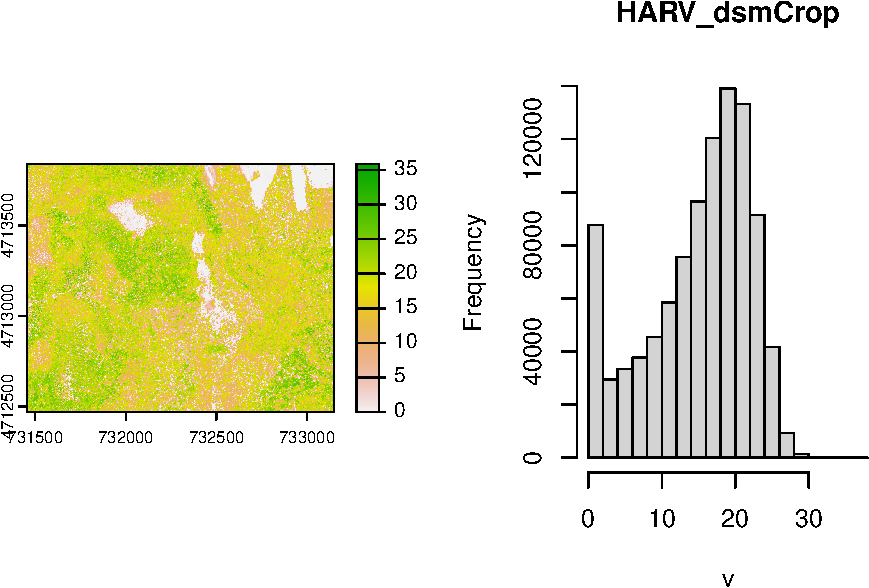
\includegraphics{R-spatial_files/figure-latex/chm-1.pdf}

This works fine for the small rasters in this tutorial. However, the calculation above becomes less efficient when computations are more complex or file sizes become large.

Thet \texttt{terra} package contains a function called \texttt{lapp()}function to make processing more efficient. It takes two or more rasters and applies a function to them. The generic syntax is:

\begin{verbatim}
outputRaster <- lapp(x, fun)
\end{verbatim}

where x is a \texttt{SpatRasterDataset} and fun is a custom function for the operation you want to perform.

\begin{Shaded}
\begin{Highlighting}[]
\NormalTok{CHM\_ov\_HARV }\OtherTok{\textless{}{-}} \FunctionTok{lapp}\NormalTok{(}\FunctionTok{sds}\NormalTok{(}\FunctionTok{list}\NormalTok{(HARV\_DSM, HARV\_DTM)), }
                    \AttributeTok{fun =} \ControlFlowTok{function}\NormalTok{(r1, r2) \{ }
                      \FunctionTok{return}\NormalTok{( r1 }\SpecialCharTok{{-}}\NormalTok{ r2) }
\NormalTok{                      \})}
\end{Highlighting}
\end{Shaded}

As arguments for our \texttt{lapp} operation we use the \texttt{sds()} function and provide it with the list of rasters that we want to operate on. As custom function we provide the function with two arguments (\texttt{r1} and \texttt{r1}) that subtracts the second (\texttt{r2}) from the first (\texttt{r1}) and returns the difference. The output of \texttt{lapp} is a \texttt{SpatRaster} and we assign it to a new variable \texttt{CHM\_ov\_HARV.}

\begin{Shaded}
\begin{Highlighting}[]
\FunctionTok{par}\NormalTok{(}\AttributeTok{mfrow =} \FunctionTok{c}\NormalTok{(}\DecValTok{1}\NormalTok{, }\DecValTok{2}\NormalTok{))}
\FunctionTok{plot}\NormalTok{(CHM\_ov\_HARV)}
\FunctionTok{hist}\NormalTok{(CHM\_ov\_HARV)}
\end{Highlighting}
\end{Shaded}

\begin{verbatim}
#> Warning: [hist] a sample of 43% of the cells was used (of which 0% was NA)
\end{verbatim}

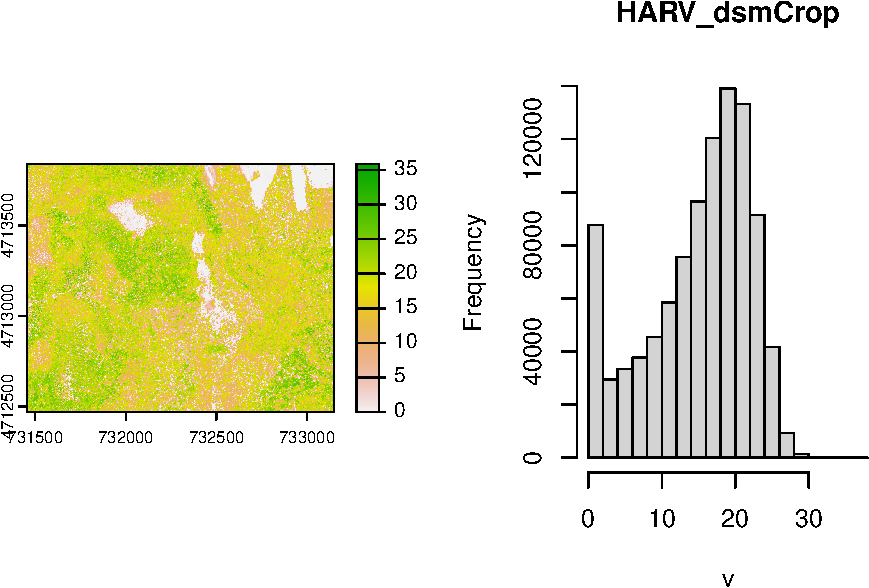
\includegraphics{R-spatial_files/figure-latex/plot-lapp-1.pdf}

\hypertarget{mapping}{%
\chapter{Making Maps in R}\label{mapping}}

\begin{quote}
Learning Objectives

\begin{itemize}
\tightlist
\item
  plot an \texttt{sf} object
\item
  create a choropleth map with \texttt{ggplot}
\item
  plot a raster map with \texttt{ggplot}
\item
  use \texttt{RColorBrewer} to improve legend colors
\item
  use \texttt{classInt}to improve legend breaks
\item
  create a choropleth map with \texttt{tmap}
\item
  plot a raster map with \texttt{tmap}
\item
  create an interactive map with \texttt{leaflet}
\item
  customize a \texttt{leaflet} map with popups and layer controls
\end{itemize}
\end{quote}

\begin{center}\rule{0.5\linewidth}{0.5pt}\end{center}

In the preceding examples we have used the base \texttt{plot} command to take a quick look at our spatial objects.

In this section we will explore several alternatives to map spatial data with R. For more packages see the ``Visualisation'' section of the \href{https://cran.r-project.org/web/views/Spatial.html}{CRAN Task View}.

\hypertarget{choropleth-mapping-with-ggplot2}{%
\section{\texorpdfstring{Choropleth Mapping with \texttt{ggplot2}}{Choropleth Mapping with ggplot2}}\label{choropleth-mapping-with-ggplot2}}

\href{http://ggplot2.org/}{\texttt{ggplot2}} is a widely used and powerful plotting library for R. It is not specifically geared towards mapping, it is possible to create quite nice maps.

For an introduction to \texttt{ggplot} check out \href{http://ggplot2.tidyverse.org/}{this site} for more pointers.

\texttt{ggplot} can plot \texttt{sf} objects directly by using the geom \texttt{geom\_sf}. So all we have to do is:

\begin{Shaded}
\begin{Highlighting}[]
\FunctionTok{library}\NormalTok{(ggplot2)}
\FunctionTok{ggplot}\NormalTok{(philly\_crimes\_sf) }\SpecialCharTok{+} 
  \FunctionTok{geom\_sf}\NormalTok{(}\FunctionTok{aes}\NormalTok{(}\AttributeTok{fill=}\NormalTok{homic\_rate))}
\end{Highlighting}
\end{Shaded}

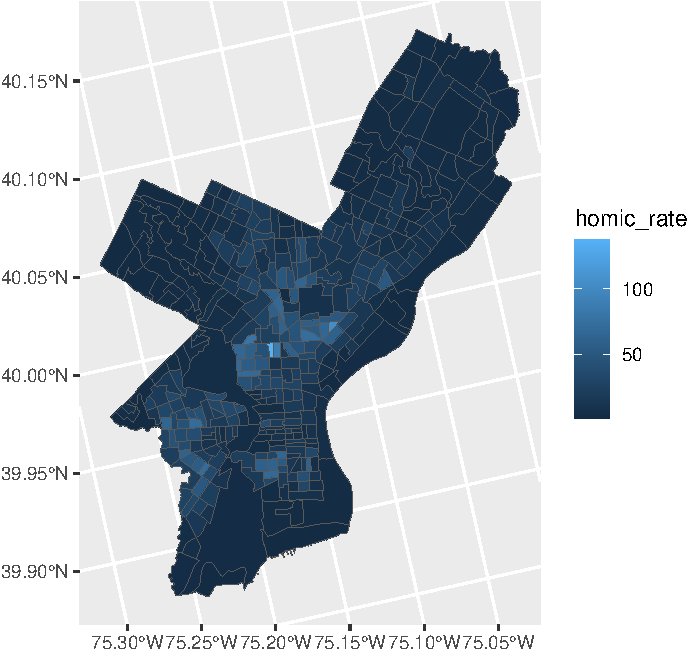
\includegraphics{R-spatial_files/figure-latex/ggplot-sf-1.pdf}

Homicide rate is a continuous variable and is plotted by \texttt{ggplot} as such. If we wanted to plot our map as a `true' choropleth map we need to convert our continous variable into a categoriacal one, according to whichever brackets we want to use.

This requires two steps:

\begin{itemize}
\tightlist
\item
  Determine the quantile breaks.
\item
  Add a categorical variable to the object which assigns each continious vaule to a bracket.
\end{itemize}

We will use the \texttt{classInt} package to explicitly determine the breaks.

\begin{Shaded}
\begin{Highlighting}[]
\FunctionTok{library}\NormalTok{(classInt)}

\CommentTok{\# get quantile breaks. Add .00001 offset to catch the lowest value}
\NormalTok{breaks\_qt }\OtherTok{\textless{}{-}} \FunctionTok{classIntervals}\NormalTok{(}\FunctionTok{c}\NormalTok{(}\FunctionTok{min}\NormalTok{(philly\_crimes\_sf}\SpecialCharTok{$}\NormalTok{homic\_rate) }\SpecialCharTok{{-}}\NormalTok{ .}\DecValTok{00001}\NormalTok{, philly\_crimes\_sf}\SpecialCharTok{$}\NormalTok{homic\_rate), }\AttributeTok{n =} \DecValTok{7}\NormalTok{, }\AttributeTok{style =} \StringTok{"quantile"}\NormalTok{)}

\FunctionTok{str}\NormalTok{(breaks\_qt)}
\end{Highlighting}
\end{Shaded}

\begin{verbatim}
#> List of 2
#>  $ var : num [1:385] 0.3 14.2 10.5 12.7 38.9 ...
#>  $ brks: num [1:8] 0.3 1.86 4.81 8.5 16.14 ...
#>  - attr(*, "style")= chr "quantile"
#>  - attr(*, "nobs")= int 385
#>  - attr(*, "call")= language classIntervals(var = c(min(philly_crimes_sf$homic_rate) - 1e-05, philly_crimes_sf$homic_rate),      n = 7, style = "quantile")
#>  - attr(*, "intervalClosure")= chr "left"
#>  - attr(*, "class")= chr "classIntervals"
\end{verbatim}

Ok. We can retrieve the breaks with \texttt{breaks\$brks}.

We use \texttt{cut} to divicde \texttt{homic\_rate} into intervals and code them according to which interval they are in.

Lastly, we can use \texttt{scale\_fill\_brewer} and add our color palette.

\begin{Shaded}
\begin{Highlighting}[]
\NormalTok{philly\_crimes\_sf }\OtherTok{\textless{}{-}} \FunctionTok{mutate}\NormalTok{(philly\_crimes\_sf, }\AttributeTok{homic\_rate\_cat =} \FunctionTok{cut}\NormalTok{(homic\_rate, breaks\_qt}\SpecialCharTok{$}\NormalTok{brks)) }

\FunctionTok{ggplot}\NormalTok{(philly\_crimes\_sf) }\SpecialCharTok{+} 
    \FunctionTok{geom\_sf}\NormalTok{(}\FunctionTok{aes}\NormalTok{(}\AttributeTok{fill=}\NormalTok{homic\_rate\_cat)) }\SpecialCharTok{+}
    \FunctionTok{scale\_fill\_brewer}\NormalTok{(}\AttributeTok{palette =} \StringTok{"OrRd"}\NormalTok{) }
\end{Highlighting}
\end{Shaded}

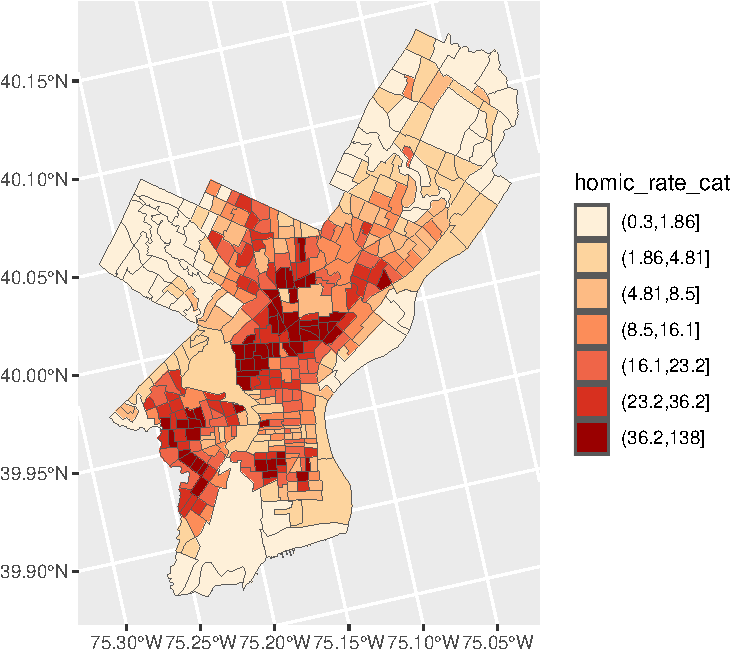
\includegraphics{R-spatial_files/figure-latex/ggplot-sf-categorical-1.pdf}

\hypertarget{raster-and-ggplot}{%
\section{Raster and ggplot}\label{raster-and-ggplot}}

To visualize raster data using \texttt{ggplot2}, we will use the raster with the values for the digital terrain model (DTM).

If you need to read it in again:

\begin{Shaded}
\begin{Highlighting}[]
\NormalTok{HARV\_DTM }\OtherTok{\textless{}{-}} \FunctionTok{rast}\NormalTok{(}\StringTok{"data/HARV\_dtmCrop.tif"}\NormalTok{)}
\end{Highlighting}
\end{Shaded}

Before using ggplot we need to convert this to a dataframe. The \texttt{terra} package has an built-in function for conversion to a plotable dataframe.

\begin{Shaded}
\begin{Highlighting}[]
\NormalTok{HARV\_DTM\_df }\OtherTok{\textless{}{-}} \FunctionTok{as.data.frame}\NormalTok{(HARV\_DTM, }\AttributeTok{xy =} \ConstantTok{TRUE}\NormalTok{)}
\FunctionTok{str}\NormalTok{(HARV\_DTM\_df)}
\end{Highlighting}
\end{Shaded}

\begin{verbatim}
#> 'data.frame':    2319798 obs. of  3 variables:
#>  $ x           : num  731454 731454 731456 731456 731458 ...
#>  $ y           : num  4713838 4713838 4713838 4713838 4713838 ...
#>  $ HARV_dtmCrop: num  389 390 389 389 389 ...
\end{verbatim}

We can now use \texttt{ggplot()} to plot this data frame. We will set the color scale to \texttt{scale\_fill\_viridis\_c} which is a color-blindness friendly color scale. \href{https://cran.r-project.org/web/packages/viridis/vignettes/intro-to-viridis.html}{Here is more about the viridis color maps.} We will also use the \texttt{coord\_fixed()} function with the default, ratio = 1, which ensures that one unit on the x-axis is the same length as one unit on the y-axis.

\begin{Shaded}
\begin{Highlighting}[]
\FunctionTok{ggplot}\NormalTok{() }\SpecialCharTok{+}
    \FunctionTok{geom\_raster}\NormalTok{(}\AttributeTok{data =}\NormalTok{ HARV\_DTM\_df , }\FunctionTok{aes}\NormalTok{(}\AttributeTok{x =}\NormalTok{ x, }\AttributeTok{y =}\NormalTok{ y, }\AttributeTok{fill =}\NormalTok{ HARV\_dtmCrop)) }\SpecialCharTok{+}
    \FunctionTok{scale\_fill\_viridis\_c}\NormalTok{() }\SpecialCharTok{+}
    \FunctionTok{coord\_fixed}\NormalTok{()}
\end{Highlighting}
\end{Shaded}

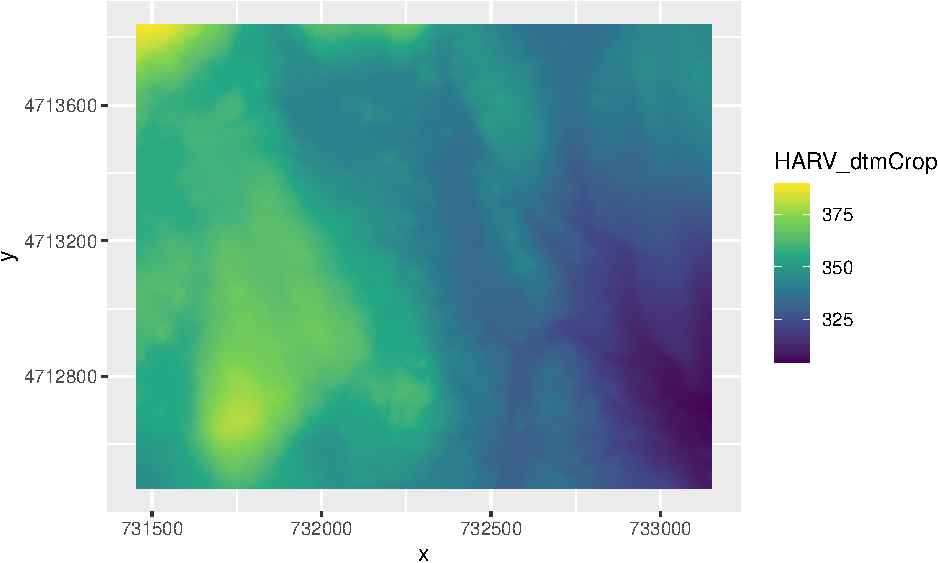
\includegraphics{R-spatial_files/figure-latex/ggplot-rast-1.pdf}

\hypertarget{choropleth-with-tmap}{%
\section{\texorpdfstring{Choropleth with \texttt{tmap}}{Choropleth with tmap}}\label{choropleth-with-tmap}}

\texttt{tmap} is specifically designed to make creation of thematic maps more convenient. It borrows from the ggplot syntax and takes care of a lot of the styling and aesthetics. This reduces our amount of code significantly. We only need:

\begin{itemize}
\tightlist
\item
  \texttt{tm\_shape()} where we provide

  \begin{itemize}
  \tightlist
  \item
    the \texttt{sf} object
  \end{itemize}
\item
  \texttt{tm\_polygons()} where we set

  \begin{itemize}
  \tightlist
  \item
    the attribute variable to map,
  \item
    the break style, and
  \item
    a title.
  \end{itemize}
\end{itemize}

\begin{Shaded}
\begin{Highlighting}[]
\FunctionTok{library}\NormalTok{(tmap)}
\FunctionTok{tm\_shape}\NormalTok{(philly\_crimes\_sf) }\SpecialCharTok{+}
  \FunctionTok{tm\_polygons}\NormalTok{(}\StringTok{"homic\_rate"}\NormalTok{, }
              \AttributeTok{style=}\StringTok{"quantile"}\NormalTok{, }
              \AttributeTok{title=}\StringTok{"Philadelphia }\SpecialCharTok{\textbackslash{}n}\StringTok{homicide density }\SpecialCharTok{\textbackslash{}n}\StringTok{per sqKm"}\NormalTok{)}
\end{Highlighting}
\end{Shaded}

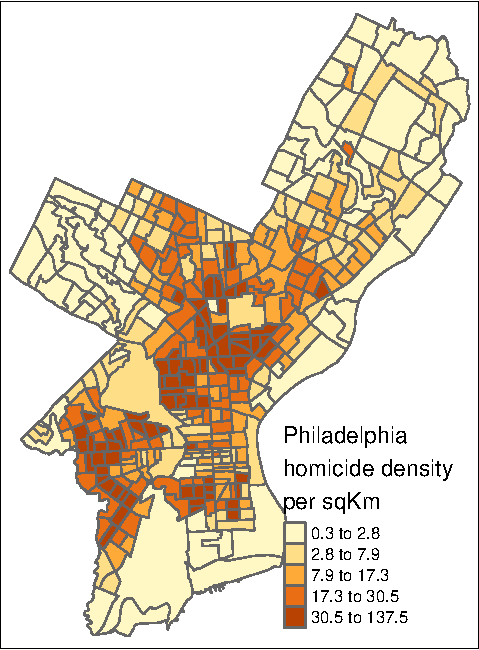
\includegraphics{R-spatial_files/figure-latex/tmap-plot-1.pdf}

\texttt{tmap} has a very nice feature that allows us to give basic interactivity to the map. We can switch from ``plot'' mode into ``view'' mode and call the last plot, like so:

\begin{Shaded}
\begin{Highlighting}[]
\FunctionTok{tmap\_mode}\NormalTok{(}\StringTok{"view"}\NormalTok{)}
\FunctionTok{tmap\_last}\NormalTok{()}
\end{Highlighting}
\end{Shaded}

Cool huh?

The \texttt{tmap} library also includes functions for simple spatial operations, geocoding and reverse geocoding using OSM. For more check \texttt{vignette("tmap-getstarted")}.

\hypertarget{raster-with-tmap}{%
\section{\texorpdfstring{Raster with \texttt{tmap}}{Raster with tmap}}\label{raster-with-tmap}}

\texttt{tmap} can also plot raster files natively, for example:

\begin{Shaded}
\begin{Highlighting}[]
\FunctionTok{tmap\_mode}\NormalTok{(}\StringTok{"plot"}\NormalTok{)}
\end{Highlighting}
\end{Shaded}

\begin{verbatim}
#> tmap mode set to plotting
\end{verbatim}

\begin{Shaded}
\begin{Highlighting}[]
\FunctionTok{tm\_shape}\NormalTok{(HARV\_DTM)}\SpecialCharTok{+}
    \FunctionTok{tm\_raster}\NormalTok{(}\AttributeTok{style =} \StringTok{"cont"}\NormalTok{, }\AttributeTok{palette =} \StringTok{"viridis"}\NormalTok{)}\SpecialCharTok{+}
    \FunctionTok{tm\_layout}\NormalTok{(}\AttributeTok{legend.outside =} \ConstantTok{TRUE}\NormalTok{)}
\end{Highlighting}
\end{Shaded}

\begin{verbatim}
#> stars object downsampled to 1114 by 897 cells. See tm_shape manual (argument raster.downsample)
\end{verbatim}

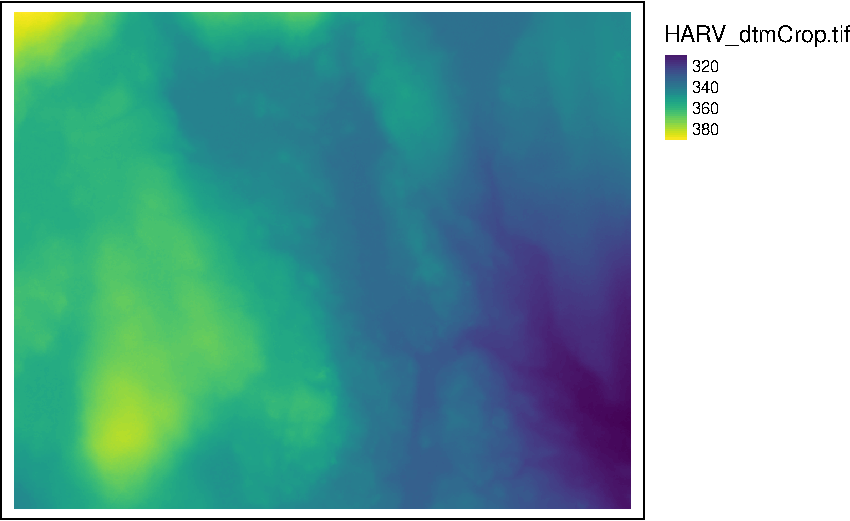
\includegraphics{R-spatial_files/figure-latex/unnamed-chunk-11-1.pdf}

See \href{https://r-tmap.github.io/tmap-book/}{Elegant and informative maps with \texttt{tmap}} for more options.

\hypertarget{web-mapping-with-leaflet}{%
\section{\texorpdfstring{Web mapping with \texttt{leaflet}}{Web mapping with leaflet}}\label{web-mapping-with-leaflet}}

\texttt{leaflet} provides bindings to the \href{http://leafletjs.com}{`Leaflet' JavaScript library}, ``the leading open-source JavaScript library for mobile-friendly interactive maps''. We have already seen a simple use of leaflet in the \texttt{tmap} example.

The good news is that the \texttt{leaflet} library gives us loads of options to customize the web look and feel of the map.

The bad news is that the \texttt{leaflet} library gives us loads of options to customize the web look and feel of the map.

Let's build up the map step by step.

First we load the \texttt{leaflet} library. Use the \texttt{leaflet()} function with an \texttt{sp} or \texttt{Spatial*} object and pipe it to \texttt{addPolygons()} function. It is not required, but improves readability if you use \href{https://github.com/tidyverse/magrittr}{the pipe operator \texttt{\%\textgreater{}\%}} to chain the elements together when building up a map with \texttt{leaflet}.

And while \texttt{tmap} was tolerant about our AEA projection of \texttt{philly\_crimes\_sf}, \texttt{leaflet} does require us to explicitly reproject the \texttt{sf} object.

\begin{Shaded}
\begin{Highlighting}[]
\FunctionTok{library}\NormalTok{(leaflet) }

\CommentTok{\# reproject}
\NormalTok{philly\_WGS84 }\OtherTok{\textless{}{-}} \FunctionTok{st\_transform}\NormalTok{(philly\_crimes\_sf, }\DecValTok{4326}\NormalTok{)}

\FunctionTok{leaflet}\NormalTok{(philly\_WGS84) }\SpecialCharTok{\%\textgreater{}\%}
  \FunctionTok{addPolygons}\NormalTok{()}
\end{Highlighting}
\end{Shaded}

To map the homicide density we use \texttt{addPolygons()} and:

\begin{itemize}
\tightlist
\item
  remove stroke (polygon borders)\\
\item
  set a fillColor for each polygon based on \texttt{homic\_rate} and make it look nice by adjusting fillOpacity and smoothFactor (how much to simplify the polyline on each zoom level). The fill color is generated using \texttt{leaflet}'s \texttt{colorQuantile()} function, which takes the color scheme and the desired number of classes. To constuct the color scheme \texttt{colorQuantile()} returns a function that we supply to \texttt{addPolygons()} together with the name of the attribute variable to map.\\
\item
  add a popup with the \texttt{homic\_rate} values. We will create as a vector of strings, that we then supply to \texttt{addPolygons()}.
\end{itemize}

\begin{Shaded}
\begin{Highlighting}[]
\NormalTok{pal\_fun }\OtherTok{\textless{}{-}} \FunctionTok{colorQuantile}\NormalTok{(}\StringTok{"YlOrRd"}\NormalTok{, }\ConstantTok{NULL}\NormalTok{, }\AttributeTok{n =} \DecValTok{5}\NormalTok{)}

\NormalTok{p\_popup }\OtherTok{\textless{}{-}} \FunctionTok{paste0}\NormalTok{(}\StringTok{"\textless{}strong\textgreater{}Homicide Rate: \textless{}/strong\textgreater{}"}\NormalTok{, philly\_WGS84}\SpecialCharTok{$}\NormalTok{homic\_rate)}

\FunctionTok{leaflet}\NormalTok{(philly\_WGS84) }\SpecialCharTok{\%\textgreater{}\%}
  \FunctionTok{addPolygons}\NormalTok{(}
    \AttributeTok{stroke =} \ConstantTok{FALSE}\NormalTok{, }\CommentTok{\# remove polygon borders}
    \AttributeTok{fillColor =} \SpecialCharTok{\textasciitilde{}}\FunctionTok{pal\_fun}\NormalTok{(homic\_rate), }\CommentTok{\# set fill color with function from above and value}
    \AttributeTok{fillOpacity =} \FloatTok{0.8}\NormalTok{, }\AttributeTok{smoothFactor =} \FloatTok{0.5}\NormalTok{, }\CommentTok{\# make it nicer}
    \AttributeTok{popup =}\NormalTok{ p\_popup)  }\CommentTok{\# add popup}
\end{Highlighting}
\end{Shaded}

Here we add a basemap, which defaults to OSM, with \texttt{addTiles()}

\begin{Shaded}
\begin{Highlighting}[]
\FunctionTok{leaflet}\NormalTok{(philly\_WGS84) }\SpecialCharTok{\%\textgreater{}\%}
  \FunctionTok{addPolygons}\NormalTok{(}
    \AttributeTok{stroke =} \ConstantTok{FALSE}\NormalTok{, }
    \AttributeTok{fillColor =} \SpecialCharTok{\textasciitilde{}}\FunctionTok{pal\_fun}\NormalTok{(homic\_rate),}
    \AttributeTok{fillOpacity =} \FloatTok{0.8}\NormalTok{, }\AttributeTok{smoothFactor =} \FloatTok{0.5}\NormalTok{,}
    \AttributeTok{popup =}\NormalTok{ p\_popup) }\SpecialCharTok{\%\textgreater{}\%}
  \FunctionTok{addTiles}\NormalTok{()}
\end{Highlighting}
\end{Shaded}

Lastly, we add a legend. We will provide the \texttt{addLegend()} function with:

\begin{itemize}
\tightlist
\item
  the location of the legend on the map\\
\item
  the function that creates the color palette\\
\item
  the value we want the palette function to use\\
\item
  a title
\end{itemize}

\begin{Shaded}
\begin{Highlighting}[]
\FunctionTok{leaflet}\NormalTok{(philly\_WGS84) }\SpecialCharTok{\%\textgreater{}\%}
  \FunctionTok{addPolygons}\NormalTok{(}
    \AttributeTok{stroke =} \ConstantTok{FALSE}\NormalTok{, }
    \AttributeTok{fillColor =} \SpecialCharTok{\textasciitilde{}}\FunctionTok{pal\_fun}\NormalTok{(homic\_rate),}
    \AttributeTok{fillOpacity =} \FloatTok{0.8}\NormalTok{, }\AttributeTok{smoothFactor =} \FloatTok{0.5}\NormalTok{,}
    \AttributeTok{popup =}\NormalTok{ p\_popup) }\SpecialCharTok{\%\textgreater{}\%}
  \FunctionTok{addTiles}\NormalTok{() }\SpecialCharTok{\%\textgreater{}\%}
  \FunctionTok{addLegend}\NormalTok{(}\StringTok{"bottomright"}\NormalTok{,  }\CommentTok{\# location}
            \AttributeTok{pal=}\NormalTok{pal\_fun,    }\CommentTok{\# palette function}
            \AttributeTok{values=}\SpecialCharTok{\textasciitilde{}}\NormalTok{homic\_rate,  }\CommentTok{\# value to be passed to palette function}
            \AttributeTok{title =} \StringTok{\textquotesingle{}Philadelphia homicide density per sqkm\textquotesingle{}}\NormalTok{) }\CommentTok{\# legend title}
\end{Highlighting}
\end{Shaded}

The labels of the legend show percentages instead of the actual value breaks\footnote{The formatting is set with \texttt{labFormat()} and in the \href{https://cran.r-project.org/web/packages/leaflet/leaflet.pdf}{documentation} we discover that: ``By default, \texttt{labFormat} is basically \texttt{format(scientific\ =\ FALSE,big.mark\ =\ \textquotesingle{},\textquotesingle{})} for the numeric palette, \texttt{as.character()} for the factor palette, and a function to return labels of the form \texttt{x{[}i{]}\ -\ x{[}i\ +\ 1{]}} for bin and quantile palettes (\textbf{in the case of quantile palettes, x is the probabilities instead of the values of breaks}).''}.

To set the labels for our breaks manually we replace the \texttt{pal} and \texttt{values} with the \texttt{colors} and \texttt{labels} arguments and set those directly using \texttt{brewer.pal()} and \texttt{breaks\_qt} from an earlier section above.

\begin{Shaded}
\begin{Highlighting}[]
\FunctionTok{leaflet}\NormalTok{(philly\_WGS84) }\SpecialCharTok{\%\textgreater{}\%}
  \FunctionTok{addPolygons}\NormalTok{(}
    \AttributeTok{stroke =} \ConstantTok{FALSE}\NormalTok{, }
    \AttributeTok{fillColor =} \SpecialCharTok{\textasciitilde{}}\FunctionTok{pal\_fun}\NormalTok{(homic\_rate),}
    \AttributeTok{fillOpacity =} \FloatTok{0.8}\NormalTok{, }\AttributeTok{smoothFactor =} \FloatTok{0.5}\NormalTok{,}
    \AttributeTok{popup =}\NormalTok{ p\_popup) }\SpecialCharTok{\%\textgreater{}\%}
  \FunctionTok{addTiles}\NormalTok{() }\SpecialCharTok{\%\textgreater{}\%}
  \FunctionTok{addLegend}\NormalTok{(}\StringTok{"bottomright"}\NormalTok{, }
            \AttributeTok{colors =} \FunctionTok{brewer.pal}\NormalTok{(}\DecValTok{7}\NormalTok{, }\StringTok{"YlOrRd"}\NormalTok{), }
            \AttributeTok{labels =} \FunctionTok{paste0}\NormalTok{(}\StringTok{"up to "}\NormalTok{, }\FunctionTok{format}\NormalTok{(breaks\_qt}\SpecialCharTok{$}\NormalTok{brks[}\SpecialCharTok{{-}}\DecValTok{1}\NormalTok{], }\AttributeTok{digits =} \DecValTok{2}\NormalTok{)),}
            \AttributeTok{title =}  \StringTok{\textquotesingle{}Philadelphia homicide density per sqkm\textquotesingle{}}\NormalTok{)}
\end{Highlighting}
\end{Shaded}

That's more like it. Finally, I have added for you a control to switch to another basemap and turn the philly polygon off and on. Take a look at the changes in the code below.

\begin{Shaded}
\begin{Highlighting}[]
\FunctionTok{leaflet}\NormalTok{(philly\_WGS84) }\SpecialCharTok{\%\textgreater{}\%}
  \FunctionTok{addPolygons}\NormalTok{(}
    \AttributeTok{stroke =} \ConstantTok{FALSE}\NormalTok{, }
    \AttributeTok{fillColor =} \SpecialCharTok{\textasciitilde{}}\FunctionTok{pal\_fun}\NormalTok{(homic\_rate),}
    \AttributeTok{fillOpacity =} \FloatTok{0.8}\NormalTok{, }\AttributeTok{smoothFactor =} \FloatTok{0.5}\NormalTok{,}
    \AttributeTok{popup =}\NormalTok{ p\_popup,}
    \AttributeTok{group =} \StringTok{"philly"}\NormalTok{) }\SpecialCharTok{\%\textgreater{}\%}
  \FunctionTok{addTiles}\NormalTok{(}\AttributeTok{group =} \StringTok{"OSM"}\NormalTok{) }\SpecialCharTok{\%\textgreater{}\%}
  \FunctionTok{addProviderTiles}\NormalTok{(}\StringTok{"CartoDB.DarkMatter"}\NormalTok{, }\AttributeTok{group =} \StringTok{"Carto"}\NormalTok{) }\SpecialCharTok{\%\textgreater{}\%}
  \FunctionTok{addLegend}\NormalTok{(}\StringTok{"bottomright"}\NormalTok{, }
            \AttributeTok{colors =} \FunctionTok{brewer.pal}\NormalTok{(}\DecValTok{7}\NormalTok{, }\StringTok{"YlOrRd"}\NormalTok{), }
            \AttributeTok{labels =} \FunctionTok{paste0}\NormalTok{(}\StringTok{"up to "}\NormalTok{, }\FunctionTok{format}\NormalTok{(breaks\_qt}\SpecialCharTok{$}\NormalTok{brks[}\SpecialCharTok{{-}}\DecValTok{1}\NormalTok{], }\AttributeTok{digits =} \DecValTok{2}\NormalTok{)),}
            \AttributeTok{title =} \StringTok{\textquotesingle{}Philadelphia homicide density per sqkm\textquotesingle{}}\NormalTok{) }\SpecialCharTok{\%\textgreater{}\%}
  \FunctionTok{addLayersControl}\NormalTok{(}\AttributeTok{baseGroups =} \FunctionTok{c}\NormalTok{(}\StringTok{"OSM"}\NormalTok{, }\StringTok{"Carto"}\NormalTok{), }
                   \AttributeTok{overlayGroups =} \FunctionTok{c}\NormalTok{(}\StringTok{"philly"}\NormalTok{))  }
\end{Highlighting}
\end{Shaded}

If you'd like to take this further here are a few pointers.

\begin{itemize}
\tightlist
\item
  \href{http://rstudio.github.io/leaflet/}{Leaflet for R}
\item
  \href{https://CRAN.R-project.org/package=rayshader}{rayshader: Create Maps and Visualize Data in 2D and 3D}
\end{itemize}

\href{https://cengel.shinyapps.io/RioSlaveMarket/}{Here is an example} using \texttt{ggplot}, \texttt{leaflet}, \texttt{shiny}, and \href{http://rmarkdown.rstudio.com/flexdashboard/}{RStudio's flexdashboard} template to bring it all together.

  \bibliography{book.bib,packages.bib}

\end{document}
